\label{chap:political_sides}

\section{\statusorange Introduction}

% In this chapter we investigated the persuasion techniques. But we have not studied the relationship between this observed persuasion in the text and the ideals/agenda/perspective of the author/outlet. It can be really useful to understand the context around the source of an article in order to interpret its persuasion.
% For this reason, the next chapter will consider perspectives and political sides. In this way we will try to understand if the persuasion of each political side is similar or which are the differences. If a different goal for the persuasion also can be observed on the persuasion itself.

In this new chapter, we introduce a new factor in our analysis.
Having in the previous one covered persuasion and propaganda, we demonstrated the need to understand the context around the source of an article in order to interpret its persuasion means.

For this reason, this chapter introduces the factor of \emph{perspectives and political sides}.
Our goal is to see and understand how persuasion (and more specifically propaganda) varies across the political spectrum. If political points of view of the sources can be so diverse, what are the techniques that they use differently in news articles to persuade the readers? Is there a link between the political orientation and the persuasion used?
% How does political point of view influence the usage of propaganda?

% Perspectives and Political Sides. What drives  the variations and propaganda? Which political interests? 

Our Research Questions for this chapter are:
\begin{itemize}
    \item RQ1: How does persuasion vary across the political spectrum?
    \item RQ2: Can we predict the political leaning of a news article by observing the propaganda it uses?
    \item RQ3: Is Propaganda Detection balanced? Or is there some imbalance in the datasets used in the literature?
\end{itemize}

The difference of terminology between the first RQ and the second RQ is due to the exclusion of sentiment when we reply to the first RQ, therefore we only indicate propaganda from there onwards.

% \todo{list contributions of this chapter}
In this chapter, we find that:
\begin{enumerate}
    \item Persuasion is used by every political leaning. With sentiment, it is more difficult to find differences as the statistical distributions are quite similar across political leaning. With propaganda, we see different usage in the quantities of techniques used in the articles, and also some term differences between left and right.
    \item By looking at propaganda features only, it is quite difficult to recognise the leaning of a news article. However, when combining the propaganda features together with the baseline features, we can improve slightly the results (but not significantly)
    \item Propaganda datasets are very unbalanced. Most of the annotated sources and articles are coming from the political right. This may cause problems in the detection of left-leaning propaganda. With unbalanced models, we still detect left-leaning propaganda, but we have no idea whether the detection is accurate.
\end{enumerate}

For this chapter, we follow the structure from the previous one~\ref{chap:linguistic_persuasion}:
\begin{itemize}
    \item first, in Section~\ref{sec:ps_political_sides}, we introduce the new ingredient: political leaning. We describe the datasets in use and the task of political leaning prediction;
    \item then, in Section~\ref{sec:ps_prop_and_leaning}, we combine the analysis of political leaning with the analysis of the previous chapters. More in specific, we analyse the relationship between propaganda and political leaning. This is the core of this experimental chapter.
\end{itemize}


\section{\statusred Political Leaning Prediction}
\label{sec:ps_political_sides}

First of all, we are taking again the definition of political leaning given in Chapter~\ref{sec:lit_leaning}: 

As we already described in the literature chapter~\ref{sec:lit_leaning}, 

\subsection{Political Leaning Definition}
\label{ssec:ps_leaning_def}

From literature

Political leaning over Left/Right axis: Left/Right definitions

Points from Left and Right ideologies (inspired by AllSides and Wikipedia and cite others) 

Disclaimer US vs the rest?

Several axes when describing news sources: L/R, factuality, 

\subsection{Datasets for Political Leaning Prediction}
\label{ssec:ps_leaning_data}

Having the task of political leaning prediction, the practical definition of leaning comes from the datasets that have been used.
For our analysis on the leaning, we have selected two resources because they are:
\begin{enumerate}
    \item publicly available
    \item relatively large: we need a good number of articles (e.g. ~) 
    \item directly indicate the political leaning of the source/articles
\end{enumerate}

Datasets annotating sources:

- MBFC
- AllSides

Datasets of articles? Is article always considered with the same leaning as source?

Details of the AllSides dataset: leaning of the author instead of the leaning of the news outlet (example).

The work by~\cite{baly2020we} mentions that the annotations are defined on the article level. But in reality, we found that from the dataset all the articles from a specific source have the same leaning annotation. ??? TRUE? OR author level?


% FROM TTO2019
FROM TTO2019
The dataset we use is from~\citet{baly2020we}, and consists of articles in English language from over 800 sources (majority from the US),\footnote{\url{https://www.allsides.com/media-bias/media-bias-ratings}} labelled for their political leaning (Left, Centre or Right).\footnote{AllSides sources: \url{https://github.com/ramybaly/Article-Bias-Prediction}}
This dataset contains several attributes for each article: full text, political leaning, topic, news source, and author name. However, in our models and experiments, we only use the text of the articles to avoid bias associated with the other attributes.
The topic distribution of the articles is uniform across the political leanings, because the dataset comes from triples of articles, one from each political leaning, about the same issue. 
% Authors of this paper publicly provide a dataset, collected from AllSides, where individual articles are labelled for their political leaning.
Note that there is a discrepancy between the description of the dataset contained in its reference paper and the dataset made publicly available by the authors on GitHub.
The dataset described in ~\citet{baly2020we} contains 34,737 articles, whereas in GitHub it has 37,554 articles (12,590 Left, 10,285 Centre, 13,399 Right).
The dataset contains two pre-splitted folds for training and testing:
\begin{itemize}
    \item \texttt{Random}: where splits are randomly generated. This classification model might encounter articles from the same media source during both training and testing phases. 
    \item \texttt{Media}; where the articles in the test set are from media sources that do not occur in the training set. %, which is more appropriate for article-based political leaning analysis. 
\end{itemize}

The Media split enables testing the classifier with less potential bias to previously seen sources, which is not the case with the Random split. Although the political-leaning of articles could sometimes be gauged by their sources, there are many examples where articles' political leaning differ from that of their sources, or the sources' leanings are not well known, or the sources themselves are unknown. Hence there is a need for such a detection to be independent of where an article came from.      
%and alignment.

\subsection{Models for Political Leaning Prediction}
\label{ssec:ps_leaning_models}

How it is computed

Usual features

State of the Art

Problems: learning the source instead of learning L/R task

\subsection{Our datasets}
\label{ssec:ps_leaning_our_data}

Is this subsection necessary? Are we doing different datasets from the others? NO --> remove

\subsection{Political leaning classification experiment}
\label{ssec:ps_leaning_classifier}

Understanding the implicit political leaning of news articles could be seen as an indicative factor for identifying misinformation~\citep{spezzano2021s}. ???

Our reproduction of classification from text (baselines):
- TF-IDF
- BERT

FROM CIMPLE

Baseline for article-level political leaning is~\citet{baly2020we}, which is the current state of the art for general purpose political leaning classification. Since the source code for this work is yet to be released, we reproduced the architecture of the model by following the details provided by the authors. Note, however, that the results we reproduced differ from those reported in their paper. This could be because of possible slight reimplementation discrepancies, and of the difference between the dataset reported in their paper and the one they shared on GitHub. Table 6 shows the results we reproduced, which form our baseline (Baly-baseline).
We embed the articles in our dataset with a pre-trained BERT model (110M parameters, uncased5) and use the vectors from the second-to-last layer, as in~\citet{baly2020we}.

\begin{table}[!htbp]
    \centering
   \scriptsize
  %\small
    % \resizebox{\textwidth}{!}{
    \begin{tabular}{l|rr|rr}
        & \multicolumn{2}{c}{Random} & \multicolumn{2}{c}{Media} \\
        Model & F1-Macro & Accuracy & F1-Macro & Accuracy \\
        \hline
        \texttt{Majority} & 21.0286 & 46.0769 & 21.0286 & 46.0769 \\
        % \texttt{Baly-API} & 42.3355 & 43.8356 & 42.0523 & 43.6910 & 41.6863 & 41.7993 & & & & \\
        \texttt{Baly-baseline} (0) & \textbf{56.4447} & \textbf{58.6153} & 40.8647 & 46.2307 \\
        \texttt{Baly-paper} (*) & 80.19 & 79.83 & 35.53 & 36.75 \\
        % \hline
        % \texttt{Prop-Total} (1) & 36.2966 & 42.3076 & 28.8285 & 41.5384 \\
        % \texttt{Prop-Techniques} (2) & 36.7166 & 40.6153 & 33.0682 & 40.5384 \\
        % \texttt{Prop-Total-Terms} (3a) & 42.0261 & 43.5384 & 41.5915 & 43.3076 \\
        % \texttt{Prop-Techniques-Terms} (3b) & 42.4357 & 43.2307 & 40.8192 & 41.9230 \\
        % % \texttt{Prop-words-BERT} (3) & 35.4718 & 48.2387 & 35.4718 & 48.2387 \\
        % \hline
        % (0) + (1) & 55.7786 & 57.7692 & 42.1847 & 47.5384 \\
        % (0) + (2) & 54.9714 & 56.9999 & 42.4362 & \textbf{47.6153} \\
        % (1) + (2) & 36.5217 & 40.4615 & 33.6202 & 41.0000 \\
        % (0) + (1) + (2) & 55.2121 & 57.1538 & 42.2102 & 47.3846 \\
        % (0) + (3a) & 54.6287 & 56.6923 & 41.9766 & 46.5384 \\
        % (0) + (3b) & 54.8004 & 56.3076 & 41.9965 & 46.2307 \\
        % (3a) + (3b) & 44.3506 & 46.3076 & 41.8725 & 44.3076 \\
        % (0) + (3a) + (3b) & 53.2549 & 54.7692 & 42.0576 & 45.92307 \\
        % (1) + (2) + (3a) & 42.0611 & 43.8461 & 42.5401 & 44.5384 \\
        % (0) + (1) + (2) + (3a) & 54.0515 & 56.0769 & 42.2358 & 46.8461 \\
        % (1) + (2) + (3b) & 44.3166 & 45.6153 & 41.9613 & 44.0000 \\
        % (0) + (1) + (2) + (3b) & 45.6153 & 45.6153 & 41.9292 & 46.2307 \\
        % (1) + (2) + (3a) + (3b) & 45.0456 & 47.2307 & \textbf{43.4564} & 45.9230 \\
        % (0) + (1) + (2) + (3a) + (3b) & 53.6459 & 53.6459 & 42.5509 & 46.5384 \\
        
    \end{tabular}
    % }
    \caption{Results given by two different baselines and the measure reported in~\citet{baly2020we}.
    }
    \label{tab:results_baselines_classifier}
\end{table}

Table~\ref{tab:results_baselines_classifier} shows the baseline results.
The line indicated with \texttt{Baly-paper} corresponds to the numbers reported in~\citet{baly2020we}.
Differences in the data and not sharing the implementation make it impossible to reproduce their baseline.
Therefore \texttt{Baly-baseline} represents our best effort in reproducing it.


Differences from baselines around?

What was learned



FROM TTO2019 VERSION

Our baseline for article-level political leaning is~\citet{baly2020we}, which is the current state of the art for general purpose political leaning classification.
% Authors of this paper publicly provide a dataset, collected from AllSides, where individual articles are labelled for their political leaning.\footnote{\url{https://github.com/ramybaly/Article-Bias-Prediction}}
Since the source code for this work has not been released yet, we reproduced the architecture of the model by following the details provided by the authors. %in~\citet{baly2020we}. 
Note, however, that the results we reproduced differ from those reported in their paper. This could be because of possible slight re-implementation discrepancies, and of the difference between the dataset reported in their paper and the one they shared on GitHub (see Section~\ref{?}), as shown in Table~\ref{tab:baly_size}.%, which is likely to be due to later updates to the dataset. 
Table~\ref{tab:results_baselines_classifier} shows the results we reproduced, which form our baseline (\texttt{Baly-baseline}). %For reference, we also include the results reported in the baseline model paper (\texttt{Baly-paper}).%, which are significant drop with the random splits while outperforming with the media splits.



% TODO table from https://github.com/ramybaly/Article-Bias-Prediction/issues/4

We embed the articles in our dataset with a pre-trained BERT model (110M parameters, uncased\footnote{\url{https://huggingface.co/google/bert_uncased_L-12_H-768_A-12}}) and use the vectors from the second-to-last layer, as in \citet{baly2020we}. %\todo{unclear} %The model is made of a single dense layer (softmax activation function) which is trained and tested with the splits provided with the dataset in~\cite{baly2020we}.

% To test our three Research Questions (Section \ref{sec:intro}), we extend the model above with various propaganda-related features, and compare their outcomes to the baseline to see if and how adding propaganda features affect the classification results.\todo{move to Experiment Setup? and clarify different between when using your model alone vs combining with basline} 


% disclaimer
Due to the small differences in the dataset and some possible differences also in the implementation of the baseline, we are not able to reproduce the results indicated as ``table 3'' of~\citet{baly2020we}. % We will substitute our implementation with the official baseline if and when its code will be shared. 

The results of Table~\ref{tab:results_rq123} show that the baseline we reproduced (\texttt{Baly-baseline}) achieves different results from the those reported in their paper (\texttt{Baly-paper}): quite significant drop with the random splits while outperforming with the media splits.
% and we are still waiting for the official code to be released (containing the implementation of their model).


%are comparing this baseline with other similar models where we use features coming from the propaganda analysis (see next) and feeding them to a model with the same single dense layer.

% that we have are going to be tested by comparing the results obtained adding specific features to the reference model. 

% For complete comparability of the results, therefore, we need to use their dataset. However, since the dataset was released only in April 2021, the experiments are also considering our own data collection from AllSides.
% At the moment, we have their dataset available (articles annotated with L/C/R labels) but we still need to finish the automated annotation of propaganda techniques (each article annotated with the 18 techniques), through an API that has quite low rate limits. For this reason we present in the following sections still the results of our own datasets (we have the propaganda annotations of them because the rate limit has been introduced only recently).


% The first dataset, here denoted with \texttt{13k} because of its size, was collected from the Headlines\footnote{\url{https://www.allsides.com/story/admin}} which are groups of three articles, usually one from the left, one from the centre and one from the right (annotated at the author level).
% This results in a dataset made of 13k articles.

% Being this dataset much smaller than the reference one, we performed a second data collection which this time considers also articles that are annotated singularly, not in groups of three as before.\footnote{\url{https://www.allsides.com/unbiased-balanced-news}}.
% This second dataset collected instead has a size of 60k articles.
% The main difference with the first one is that the articles are not grouped in triples of Left/Center/Right. This results in the 60k dataset being much more unbalanced than the 13k (which still is a bit unbalanced because not exactly all the groups keep the balance).

% The third dataset is coming from~\citet{baly2020we} through the official GitHub repository \url{https://github.com/ramybaly/Article-Bias-Prediction}. We observe that there are some differences with what is stated in their paper, as can be seen in table~\ref{tab:baly_size}. What probably happened is that the authors kept collecting more articles.

\begin{table}[]
   \centering
   \begin{tabular}{r|c|c|c}
       & train & validation & test \\
       \hline
       Paper media & 22,969 & 5,098 & 1,200 \\
       github media & 26,590 & 2,356 & 1,300 \\
       \hline
       Paper random & 26,828 & 6,709 & 1,200 \\
       github random & 27,978 & 6,996 & 1,300
   \end{tabular}
   \caption{Some of the differences between the publicly available dataset and the statistics reported in~\citet{baly2020we}}
   \label{tab:baly_size}
\end{table}

% Now, by comparing the two different datasets collected with the dataset from~\cite{baly2020we}, Figure~\ref{fig:venn} shows that the 13k and Baly are mostly balanced subsets of the 60k.
% Although the URLs of the articles in the Baly dataset are a subset of the URLs of the articles in our datasets (13k and 60k), the texts of the articles do not match: the data cleaning of \texttt{Baly} is different and better than our data cleaning (e.g. removing non-article content), and having different texts makes the propaganda annotations differ slightly.

% The last dataset considered is derived from the 60k, by keeping it balanced between target labels. Since the smaller group (Center) has 11309 articles, we limited the articles from the Left and Right to contain 11309 articles too, through random selection. We will compare the results of the unbalanced 60k with the balanced 60k.

% TODO: only table or only histogramm
% \begin{figure}[!htb]
%     \centering
%     \includegraphics[width=\columnwidth]{figures/dataset_comparison.pdf}
%     \caption{Distribution of the three datasets across the political spectrum}
%     \label{fig:dataset_comparison}
% \end{figure}

% \begin{table}[!htb]
%     \centering
%     \begin{tabular}{l|r|r|r}
%         Dataset & \#Left & \#Center & \#Right \\
%         \hline
%         13k & 6058 & 2672 & 4408 \\
%         60k & 27457 & 12565 & 20441 \\
%         60k-balanced & 12565 & 12565 & 12565 \\
%     \end{tabular}
%     \caption{Distribution of the three datasets across the political spectrum}
%     \label{tab:dataset_comparison}
% \end{table}

% \begin{figure}[!htb]
%     \centering
%     \includegraphics[width=\columnwidth]{figures/venn.pdf}
%     \caption{Overlap between the three datasets}
%     \label{fig:venn}
% \end{figure}




% - source labels vs author labels?
% \\

% classifier comparison with theirs
% Since at the moment the results are shown from our datasets, the only way to compare with the baseline is to use the same model. For this, we are waiting for their implementation to be shared. In the meanwhile, we have tried to emulate the baseline, based on the description of the model given in~\citet{baly2020we}. We name this set of results with \texttt{Baly-baseline}. However, the results of this model are lower than the official results, so there have to be other differences other than the dataset size increased.
%     \item using a prediction endpoint of political leaning exposed by the same research group. We do not know if this endpoint is an implementation of the model described in~\citet{baly2020we} or not, the results will tell. We name this set of results with \texttt{Baly-API}.
% \end{itemize}
% Instead, for the second big issue of comparability (the model), we need to have their model implementation to compare our results. While the dataset was not shared with us, this was the only possible way to compare: feed our dataset to our models and theirs and compare fairly the scores. We found that their API exposes a political leaning prediction endpoint that accepts sending text and provides the probability of the article to belong to left/center/right. We don't know if this implementation is the one behind the paper (the prediction belongs to the same project at QCRI) but we assume it is.
% Therefore we sent all the articles that we have in our datasets to that endpoint and took the argmax of that prediction. The results collected with this method are annotated here with \texttt{Baly-API}.
% From the description given in their paper~\cite{baly2020we} we tried to reproduce locally the same model. We will observe how much this is the same with the results of \texttt{Baly-API}. These results are annotated with \texttt{Baly-baseline}.
% As soon as the implementation of the model will be shared by the authors, this confusion will be removed.
% \\


\section{\statusorange Persuasion and Political Leaning Prediction}
\label{sec:ps_prop_and_leaning}

Here we want to see the relationship between Persuasion (studied in the previous Chapter~\ref{ssec:lp_techniques_propaganda} and Political Leaning (from the previous Section~\ref{sec:ps_political_sides}).
This is the core of this chapter as it analyses the relationship between persuasion and leaning. In the previous Chapter~\ref{chap:linguistic_persuasion} we analysed persuasion on its own
For this reason, we are combining the two analyses with the following experiments:

\begin{enumerate}
    \item Analysis of persuasion features across the political spectrum: we want to understand if we can see some difference between the persuasion means of left, center and right (Section~\ref{ssec:ps_prop_leaning_across}). We are able to identify some differences both in the quantity of specific techniques, and in the terms used.
    \item Prediction of the political leaning using persuasion features. Can machine learning models differentiate between propaganda and sentiment from left and right? (Section~\ref{ssec:ps_prop_leaning_classifier}) The motivation of this experiment is that we are able to see some differences from the previous experiment, and therefore we want to see if also machine learning classifiers can differentiate and how well. We find that it is possible to classify the leaning of news articles based on their use of propaganda, but that it is quite hard to be better than classifiers based on the full text of the articles. 
    \item Are the current propaganda datasets unbalanced? (Section~\ref{ssec:ps_prop_leaning_unbalanced}). Given that the results of both previous experiments (manual and automated) are dependent on the quality of the automated propaganda detection, in this last experiment of the chapter we do an analysis of the imbalance of the data that was used to train the propaganda detector. We find that in most of the cases, propaganda examples come from Right-leaning sources and the Left and Center are underrepresented.
\end{enumerate}

\subsection{\statusgreen Persuasion across the political spectrum}
\label{ssec:ps_prop_leaning_across}
% From Experiment 4.3: comparison of sentiment/propaganda across political leaning

Our first RQ for this chapter is: \emph{How does persuasion vary across the political spectrum?}

To answer this question, we perform a comparison across the political leanings to see if we can identify major differences (for example, one leaning could contain more of one specific technique, or differentiate in the terms used).
For this reason, we perform the comparison by considering both the \emph{amount} of each persuasion technique, and the \emph{term frequencies}.

% - overall sentiment and propaganda across spectrum
%     - quantities
%     - terms
% - for each technique, what are the variations
%     - quantities
%     - terms


Our hypothesis is that more extreme views will contain more persuasion (especially propaganda techniques). This might be the case because stronger positions are characteristic of the extremes, while moderate and center views may express news in a more neutral way, less filled with persuasion.

\subsubsection{Dataset}
% dataset
The dataset used is AllSides, as in the previous experiments.
We take from it the text of the articles and the label for the leaning, expressed over 3 distinct values: Left Center, Right
%, Mixed, Not Rated. The first 5 values are properly placed across the spectrum, from left to right. The last values instead are for data that is not clearly aligned with one leaning.
It is important to note that the articles in this dataset are grouped in triples covering the same story, and this grouping makes the topic perfectly balanced across the dataset. For each article belonging to one leaning, there exist two other articles that belong to the other two leanings.
In this way, we do not need to consider the fact that some topics may naturally be more subject to persuasion (e.g. political issues) while other topics may be less (e.g. sports or technology, where the writing style could be less loaded).
Having this link between the articles in the dataset allows us to focus on the comparative results excluding the variable of the topic (for now, but we will introduce the topic as a variable in the next Chapter~\ref{chap:topics}).

% features extraction: sentiment/propaganda
From the text of each of the articles, we then extract the persuasion techniques (sentiment and propaganda, as in the previous Chapter~\ref{sec:lp_techniques}). This gives us for each document a set of words annotated with the corresponding technique. From these annotated words, we compute two features:
\begin{enumerate}
    \item word-based percentage of each technique
    \item terms for each technique
\end{enumerate}


% 1. Extraction of propaganda/sentiment
% Each article is analysed independently from the others, using the propaganda detection method and the sentiment lexicons.
% The percentages of words annotated with respect to the total number of words are computed for each article.

% 2. Grouping the percentages by political bias
We then consider the labels given by AllSides (left, center, right), and we aggregate the average of word-based percentages (mean, quartiles, distribution). %This gives an idea of how much of the articles from each political side is detected as sentiment-related or propaganda-related.
We also aggregate the term distributions to compute the term relative importance (TF-IDF) to then try to understand if the left, center and right are using different words to express their persuasion.

\subsubsection{Comparison of the quantity of persuasion across leanings}

\begin{figure}[!htbp]
    \centering
    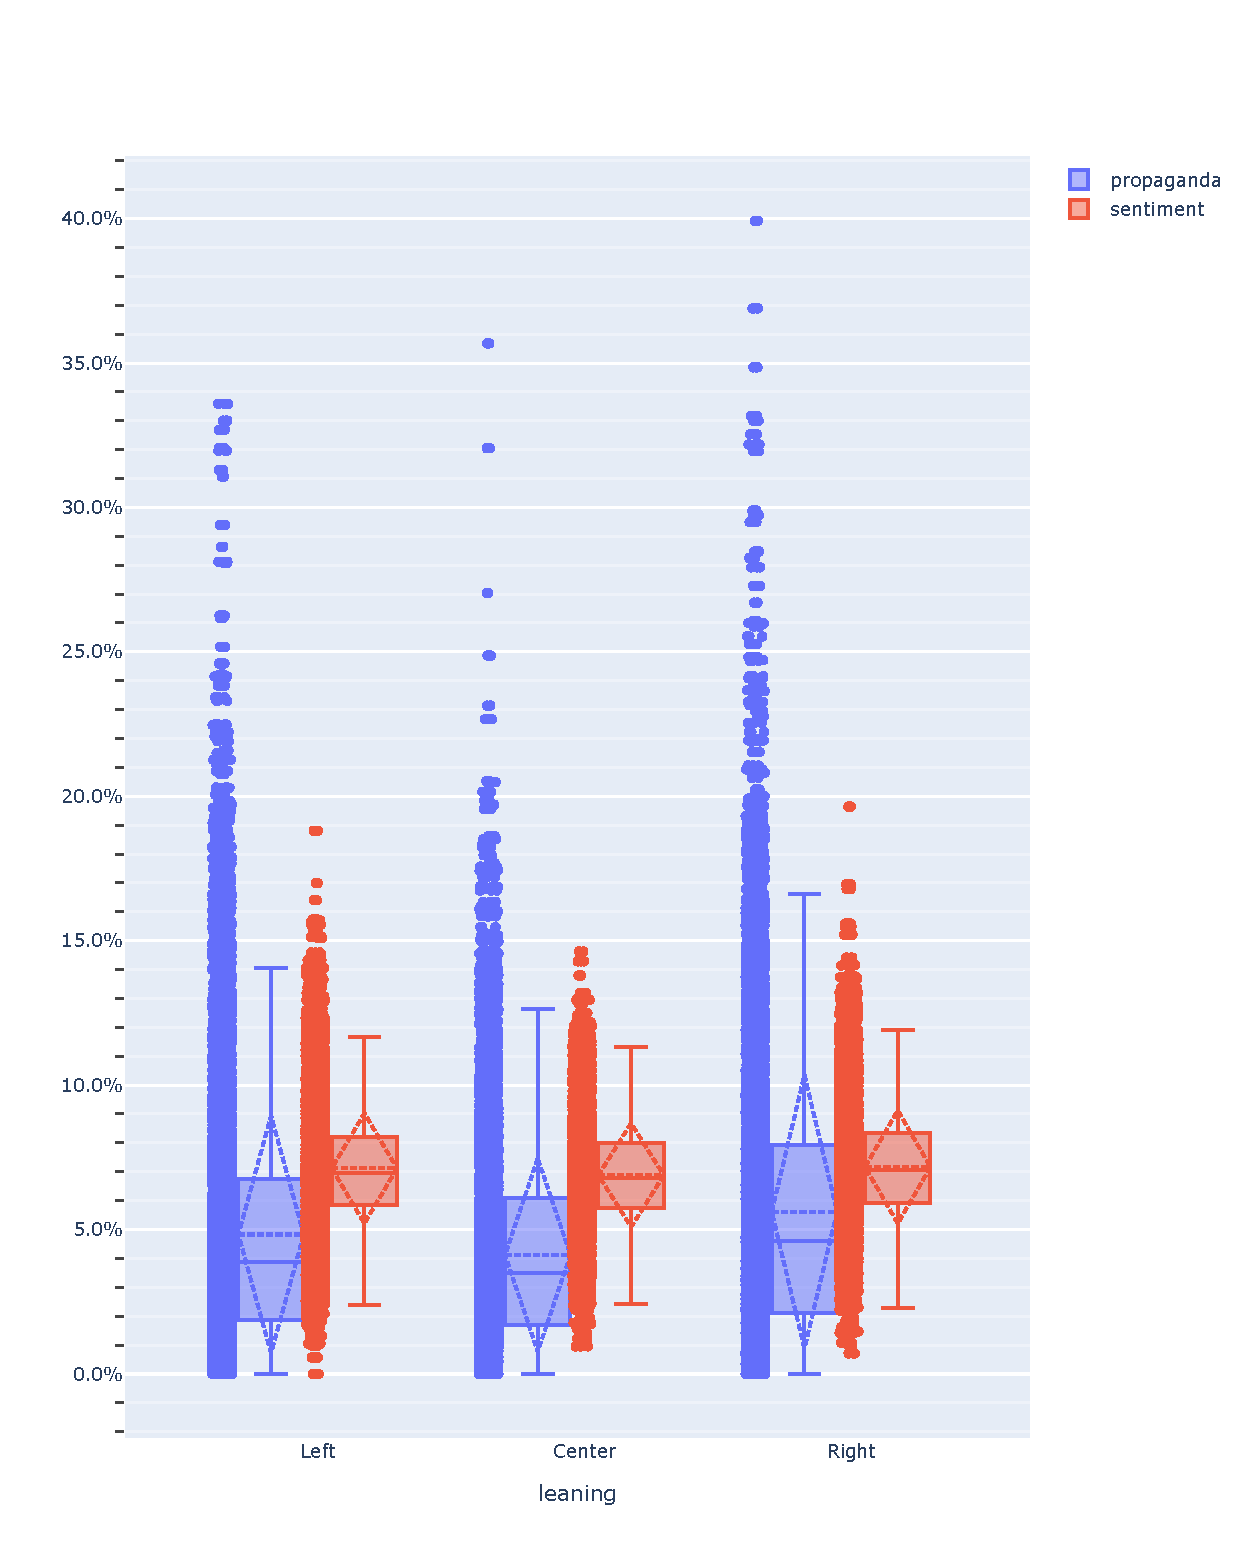
\includegraphics[width=\linewidth]{figures/prop_sent_tech_across_leaning_headlines_mod.pdf} % features_by_bias_box_cleaned_all.pdf
    \caption{Comparison of the detected sentiment and propaganda across the political leaning (horizontal axis). On the vertical axis, the average of the word-based percentage is represented. The boxes represent Q1 (25\% quartile) Q2 (median) and Q3 (75\% quartile). The diamond represents mean and standard deviation, while the whiskers are drawn within the 1.5 IQR value.}
    \label{fig:prop_sent_across_leaning}
\end{figure}


Figure~\ref{fig:prop_sent_across_leaning} is a representation (with data points on the left, and the boxplot with quartiles on the right) which shows the distribution of the ratios computed. We can see that for sentiment, we have very similar average values and distributions (median, Q1, Q3, mean).
For this reason, we conclude that sentiment is not a good indicator of the differences between political leanings. We cannot find any differences between left and right.

Instead, when we consider propaganda, we see that on the Right we have more words detected as propagandistic.
The Center has slightly fewer words detected in propaganda with respect to the other two leanings (mean values Center=$4.1\%$, Left=$4.9\%$, Right=$5.6\%$).
This confirms our hypothesis that the center contains less propaganda than more polarised political leanings.

% We did a c

% From this plot we see that there are some very strange values (76\% of highlighted words in one article from the center). Looking at the details, this is an article from BBC which does not look so subjective. The problem is that from the full article, the scraping library only captured the sentence The statement says: ``It is an assault on UK sovereignty and any such use by a State party is a clear violation of the Chemical Weapons Convention and a breach of international law. It threatens the security of us all." which is annotated as almost everything propaganda. For other BBC articles, scraping manages to retrieve the full text without problems.

% There are also a lot of articles which have a percentage of 0\%. Looking at the distribution of the length of the documents, some documents, especially from some sources, have length=0 or a very short length (scraping the cookie disclaimer instead of the full article).
% For this reason a minimum length threshold has been set to cut out these problems: 150 tokens at least.

% This is the same plot, but with the filter on the minimum length.
% We can see that:
% The most annotated side is the Right
% The least annotated side is the Left
% Article from the Center do not contain less sentiment/propaganda (against assumption)
% There are fewer propaganda words than sentiment words

% BREAKDOWN BY TECHNIQUE
We then analyse more in detail the breakdown by specific propaganda technique. For this, we keep separated the word-based percentages for each technique.
Our aim is to see whether some techniques are used more in one specific leaning than in the others.


\begin{figure}[!htbp]
    \centering
    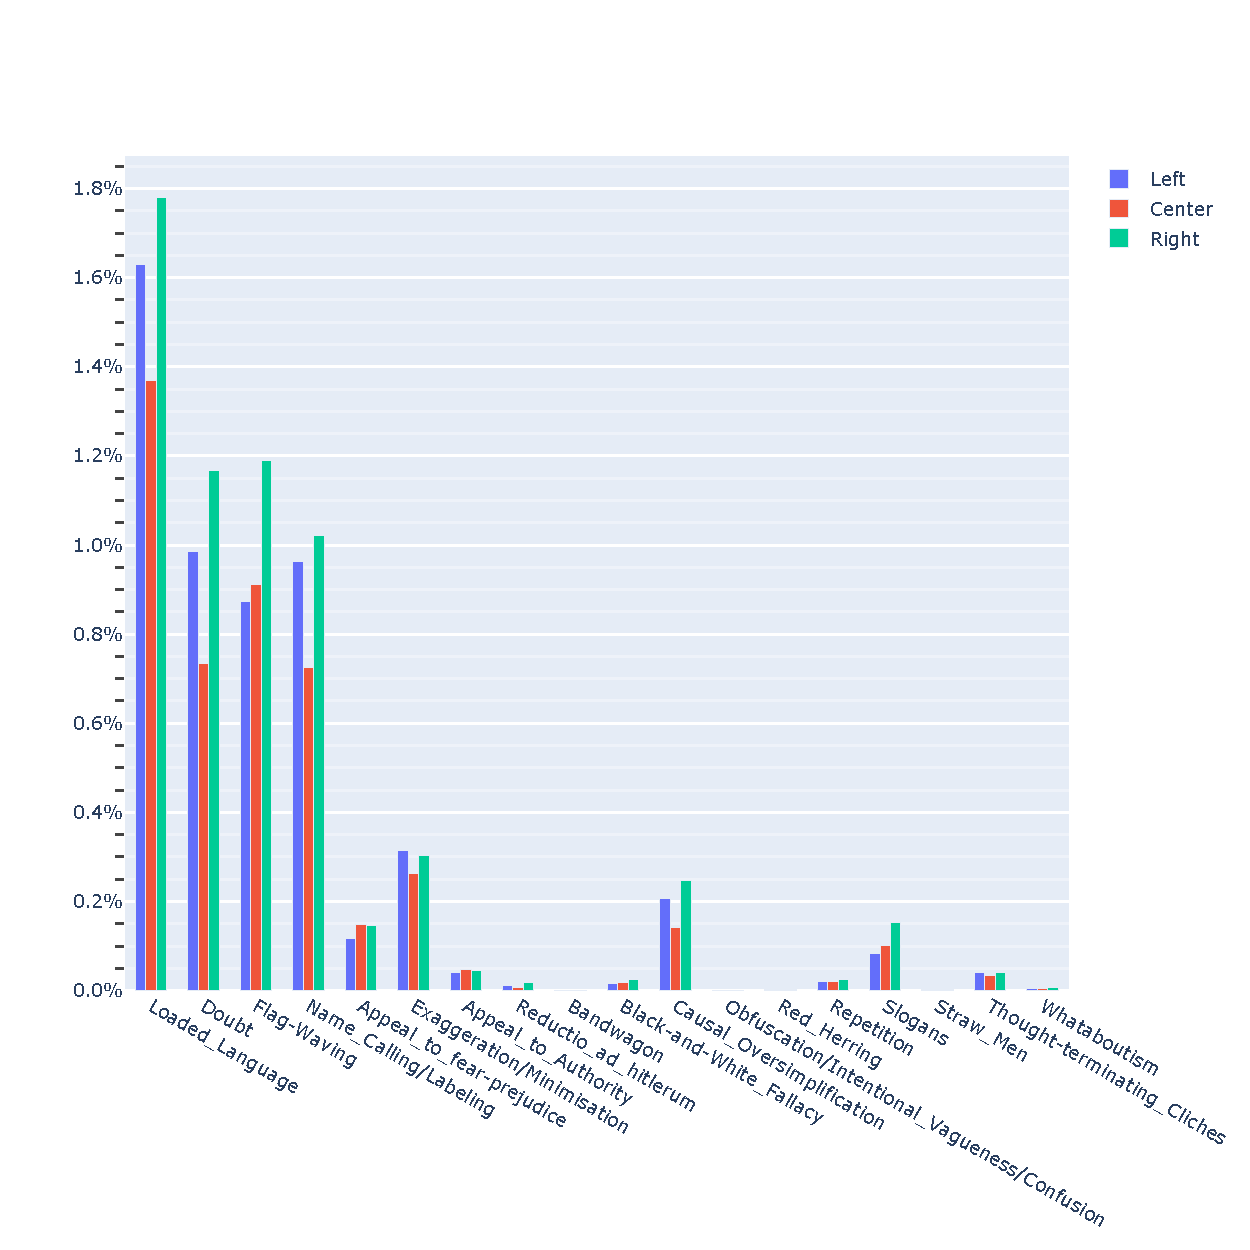
\includegraphics[trim={0 0 0 2cm},clip,width=\linewidth]{figures/prop_tech_detail_across_leaning_baly.pdf}
    \caption{Breakdown of propaganda techniques by political leaning.}
    \label{fig:prop_tech_details_across_leaning}
\end{figure}
\todo{Would it be better to show also std deviation or other distribution info like in the previous plot?}

Figure~\ref{fig:prop_tech_details_across_leaning} shows on the vertical axis the different propaganda techniques, and each colour represents a different political leaning. The vertical axis represents the mean word-based percentage of the specific propaganda technique for the considered leaning.
With this plot we can compare the techniques across the leanings.

First of all, we notice that the most common propaganda techniques are \texttt{Loaded\_Language}, \texttt{Doubt}, \texttt{Flag-Waving} and \texttt{Name\_Calling/Labeling}.
The articles in the dataset contain on average $1.5$ loaded terms every $100$ words.

% shape analysis
We can see different types of patterns in this plot, which are shown with different shapes over the leanings.
% U-shape
The first one, that we call \emph{U-shape}, happens when the bars of the Left and Right are higher than the bar of the Center. This means that what is represented is polarised on the extremes of the political spectrum.
A good example of this type is the \texttt{Loaded\_Language}, where the Center is using this technique on $1.38\%$ of the words, while Left and Right are using it considerably more.
The same happens with \texttt{Doubt}, \texttt{Name\_Calling/Labeling}, \texttt{Exaggeration/Minimisation}, \texttt{Causal\_Oversimplification}.
These techniques are used by more extreme articles and are giving the general trend that we observed in the previous Figure~\ref{fig:prop_sent_across_leaning}: the center is more moderate and uses less them.

% triangular shape
A second pattern that we notice, is the \emph{triangular shape}. In this shape, the quantities of the technique considered increase (\emph{triangular Right}) or decrease (\emph{triangular Left}) monotonically when going from Left to Right leaning.
This behaviour means that the technique analysed is inherent of a specific extreme of the political leaning spectrum, and constantly decreases when moving to the other side.
It is not surprising that \texttt{Flag-Waving} presents this behaviour, where it is way more detected in Right-leaning articles with respect to Center and even more with Left. This technique is conceptually linked with the principles of nationality, and the strong nationalism is usually associated with Right-leaning political stance.
The same pattern occurs with \texttt{Slogans}. We can link this with the abundance of left-leaning slogans in the recent date range of the dataset for the Trump re-election campaign~\citep{jiang2020political}.

% Reversed U
Another pattern that we see, is the opposite of the first one: \emph{reversed-U shape}. This is characterised by a higher use in the Center than in the extremes.
It represents techniques that are used to moderate more and may have a balancing intent.\todomargin{?}
We can see this pattern with the techniques \texttt{Appeal\_to\_fear-prejudice} and \texttt{Appeal\_to\_authority}. While for the first one, it is unbalanced (highest value center, then Right and then quite less Left), in the second case this is more balanced (Left and Right have similar values).

\subsubsection{Comparing propaganda-term importance across leaning}
We then move to the term analysis, to see if we can find any differences in the specific terms used by each leaning.

\todo{Fix this insertion of WordClouds}
WHY JUST TERM COUNTING IS NOT ENOUGH: example from wordclouds. Similar terms, just a few are unique of the leaning. The importance of comparing distributions and IDF

\begin{figure*}[!htb]
     \centering
     \begin{subfigure}[b]{0.3\textwidth}
         \centering
         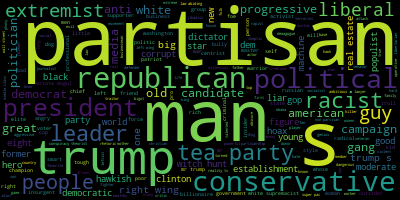
\includegraphics[width=\textwidth]{figures/baly_wordclouds_Name_Calling,Labeling_Left.png}
         \caption{Left}
         \label{fig:wc_loaded_left}
     \end{subfigure}
     \hfill
     \begin{subfigure}[b]{0.3\textwidth}
         \centering
         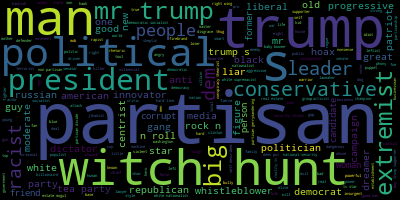
\includegraphics[width=\textwidth]{figures/baly_wordclouds_Name_Calling,Labeling_Center.png}
         \caption{Center}
         \label{fig:wc_loaded_center}
     \end{subfigure}
     \hfill
     \begin{subfigure}[b]{0.3\textwidth}
         \centering
         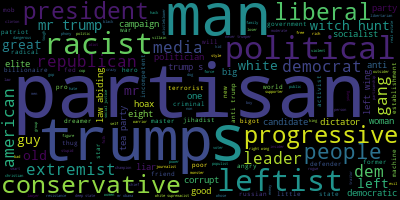
\includegraphics[width=\textwidth]{figures/baly_wordclouds_Name_Calling,Labeling_Right.png}
         \caption{Right}
         \label{fig:wc_loaded_right}
     \end{subfigure}
        \caption{WordClouds from words belonging to the \texttt{Name\_Calling} propaganda technique}
        \label{fig:wc_name_calling}
\end{figure*}

Qualitative term analysis done on the words belonging to the different political leanings in our dataset. As Figure~\ref{fig:wc_name_calling} shows, there are some differences in some of the propaganda techniques (shown from the \texttt{Name\_Calling} technique as an example):
media sources from the Left appear to frequently use ``republican'' and ``conservative'', while in the Right we can see some unique terms such as ``leftist'' and ``progressive''. Some words are equally used, possibly for different meanings, such as ``partisan''.  
Although these differences, the most repeated word from all the leanings is the word ``partisan'' which is used as a wildcard and probably is intended with different meanings.
But the effect is that most of the terms are repeated in all the leanings, and therefore we have to rely on a better concept than simply counting the term occurrences. 
This is why we use the concept of relative term importance from TF-IDF




CONTINUING WITH TF-IDF

We rely on the concept of term importance, as defined by the TF-IDF model: the importance of a term is directly proportional to how many times it appears in the considered document (Term Frequency) and inversely proportional to the number of times it appears in the whole corpus (Inverse Document Frequency).

Here, since we want to understand the relative importance of terms between political leanings, we consider as documents the concatenation of all the selected terms (from propaganda analysis) from all the articles coming from a certain leaning. In other words, we have a corpus made of 3 documents (one for Left, one for Center, one for Right).

We perform this analysis first with all the propaganda techniques together, and secondly by considering each technique separately.

% TERM ANALYSIS OVERALL
For the term importance across all the propaganda techniques, we process each article and select the detected words of propaganda that belong to any of the 18 techniques. Then we collect all these words in 3 buckets, one for each leaning.
We apply on these 3 groups the standard TF-IDF as provided by the \texttt{gensim} library (applied on lemmatised words).
This produces a matrix of weights with a shape of $[n_{features}, 3]$ (feature size x number of classes), together with the features names.

Then to identify the features that differ the most between the leanings, we ranked the features based on decreasing $(max - min)$. In this way, we get as first ones the features whose values have the maximal difference.
These features have high value for the leaning they are mostly occurring in, and lower values for the leaning where they do not appear very frequently.
We can then say that these terms are the most distinguishable propaganda terms across the political spectrum.

\begin{figure}[!htbp]
    \centering
    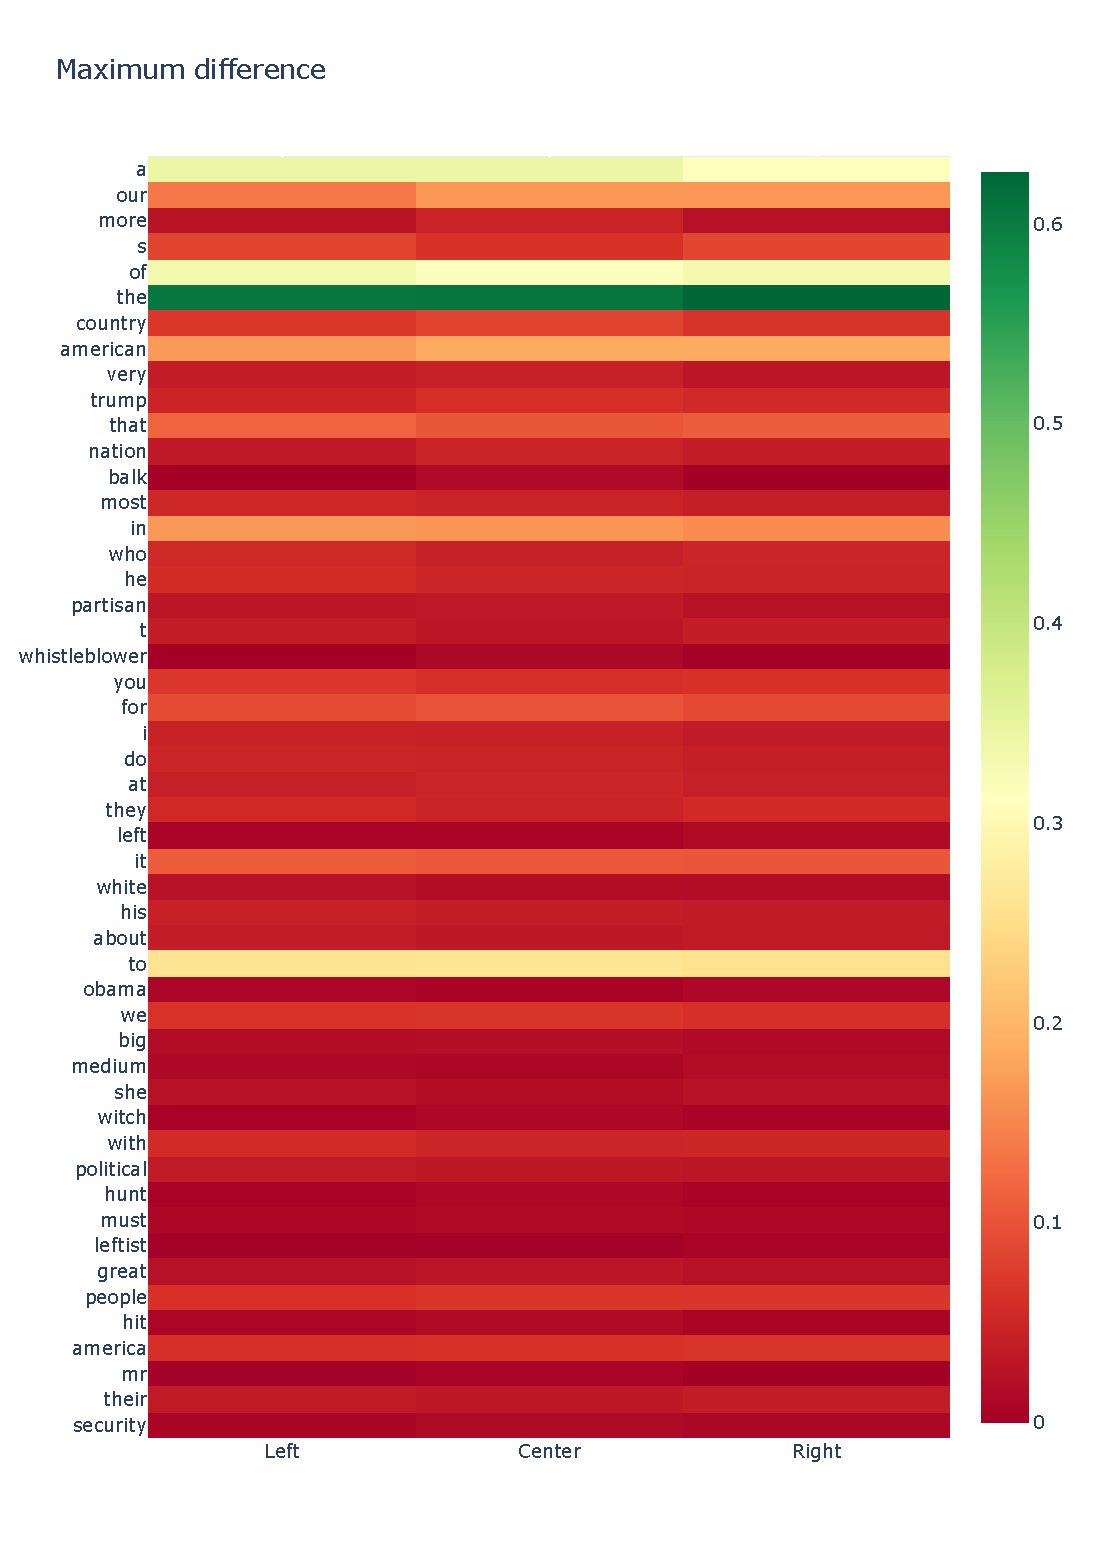
\includegraphics[trim={0 0 0 2cm},clip,width=\linewidth]{figures/baly_prop_tech_words_all_across_leaning.pdf}
    \caption{Propaganda terms with the maximum difference in TF-IDF importance across political leaning.}
    \label{fig:baly_prop_tech_words_all_across_leaning}
\end{figure}

Figure~\ref{fig:baly_prop_tech_words_all_across_leaning} shows the top 50 features (words) that have the maximal difference between the maximum and the minimum.
We did not remove stopwords because we are only dealing with some fragments of sentences that have been detected as propagandistic. For this reason the plot is showing some stopwords (e.g., ``a", ``of", ``the").
From this plot we can recognise some propaganda terms.
For example ``our" and ``american", ``leftist", ``people", ``america" that are more important for the right. From~\citet{seargeant2020art} we know that the Right is using more statements like ``we the people" which is a Right-leaning expression of populism. We also think that the appearance of ``leftist" as a pseudonym given by Right-wing to indicate Left-wing is quite meaningful.
Then we notice some terms that are more related to the center: ``country", ``trump", ``nation", ``partisan", ``whistleblower", ``great".

% TERM ANALYSIS PER TECHNIQUE
However, from this analysis, it is not clear how the terms found relate to the specific propaganda techniques. For this reason, we decide to perform again this analysis, but for each propaganda technique separately.
This means that we build the term frequencies for each of the 18 techniques, by collecting the terms that have been used in the specific technique by each leaning, and then building the TF-IDF feature separately and sorting again by the $(max - min)$ criterion.

With this method, we collect the most important words for each technique and leaning in Table~\ref{tab:prop_words_by_technique_and_leaning}.

\begin{table}[!htbp]
% \Rotatebox{90}{%
\resizebox{\textwidth}{!}{
    \centering
    \begin{tabular}{p{0.30\textwidth}|p{0.40\textwidth}|p{0.40\textwidth}|p{0.40\textwidth}}
        technique & Left & Center & Right \\
        \hline
         \texttt{Loaded\_Language} & in, that, into, self, devastating, hell & balk, more, very, whistleblower, hit, expose, batten, out, badgering, divisive, blast, circus, dramatic, chaos, severe & evil, blasted  \\
         \hline
         \texttt{Doubt} & just & trump, inadequate, transparency, grapple, will  & why, FBI, if \\
         \hline
         \texttt{Flag-Waving} & America, \textbf{white}, \textbf{black}, \textbf{life}, \textbf{society}  & democracy, state, security, family, value & \textbf{people}, \textbf{we}, \textbf{freedom}, \textbf{law}, \textbf{liberty} \\
         \hline
         \texttt{Name\_Calling/ Labeling} & party, \textbf{republican}, \textbf{right}, \textbf{conservative}, wing, real   & \textbf{partisan}, trump, witch, hunt, dems, whistleblower, innovator, dreamer, \textbf{centrist}, president, \textbf{democratic}, hoax  & \textbf{leftist}, racist, hating, law, \textbf{liberal}, \textbf{progressive}   \\
         \hline
         \texttt{Appeal\_to\_fear- prejudice} & \textbf{threat}, \textbf{climate}, difficult, death, die, disproportionate   & risk, backfire, credible, dangerous, confidence   & all, \textbf{destroy}, \textbf{attack}, fight, economically, racism, \textbf{invade}  \\
         \hline
         \texttt{Exaggeration/ Minimisation} & best, more, incredible, impossible, biggest, could, dramatically  & history, deadliest, big, unprecedented, life, degradation  & worst, absolutely, great, ever  \\
         \hline
         \texttt{Appeal\_to\_Authority} & medium, wisdom, \textbf{news}, know  & transparent, \textbf{intelligence}, official  & \textbf{note}, lie, open, \textbf{written}, accurate, fair, reflect   \\
         \hline
         \texttt{Reductio\_ad\_ hitlerum} & Stalinist, communism, partisan, & gestapo, nazi, eagle, religion, blame,   & hitler, Donald, tactic, propaganda, resurgent, science, death, gay \\
         \hline
         \texttt{Bandwagon} & find, common & say & taken, some, leave, future \\
         \hline
         \texttt{Black-and-White\_ Fallacy} & evolution, bible, proof, fall,  & impeachable, wall, good, strength, punch, military, justice, democratic, deal & my, live, change, amendment, senate \\
         \hline
         \texttt{Causal\_ Oversimplification} & plot, think & all, say, \textbf{reality}, reason, political & member, \textbf{leftist}, life, left  \\
         \hline
         \texttt{Obfuscation/ Intentional\_ Vagueness/ Confusion} & suggest, wrong, impossible, guide, evil, efficacy, anything & power, right, answer, excuse, truth, simply  & wing, meaning, rule, master, magic, fiction \\
         \hline
         \texttt{Red\_Herring} & love, pay, believe, anymore, like & & life, think, family, adulterous, America, republican, statement  \\
         \hline
         \texttt{Repetition} & jealous, blind, ObamaCare, bully, poison, lie  & more, temple, satanic, breathe & trump, obama, abiding, careless, law, pray, rigged, extremely  \\
         \hline
         \texttt{Slogans} & survival, fight, \textbf{matter}, \textbf{life}, face, \textbf{lives} & \textbf{America}, first, \textbf{great}, win, \textbf{make}, anchor, hero  & learn, amid, hearing, over, call, tax, race  \\
         \hline
         \texttt{Straw\_Men} & read, vote, opposition, trump & love, rule, poll & lie, news, god, want \\
         \hline
         \texttt{Thought-terminating\_ Cliches} & give, follow, lie  & wasting, time, drama & enough, break, evidence \\
         \hline
         \texttt{Whataboutism} & control, prison, & point, system, news, real, democrat, care  & apartheid, people, law, American, make, worse, contain \\
    \end{tabular}
}
    \caption{Terms with higher difference in TF-IDF weights for each propaganda technique across leaning.}
    \label{tab:prop_words_by_technique_and_leaning}
\end{table}

As we can see, for each propaganda techniques there are different terms that are more or less important for each leaning. While for some of these techniques, the terms are not very talkative, we can see in some cases that the results are quite meaningful.
For example, in the \texttt{Name\_Calling/Labeling} technique we can see how the different political leanings address each others: the Right addresses the Left with the term \emph{leftist}, \emph{liberal} and \emph{progressive} and never with \emph{democrats} (term used instead by the center). Instead, the Left addresses the Right with \emph{republican}, \emph{right} and \emph{conservative}.

Or for the \texttt{Flag-Waving} technique, that we see how \emph{we the people} emerges from the Right, while the Left is more about \emph{white/black} and \emph{life/society}.
Also in the \texttt{Appeal\_to\_fear-prejudice}, we can see how thematically the Right is more recognisable for terms related to invasion/attack/destruction, while the Left emerges uniquely with \emph{climate}.
For the \texttt{Appeal\_to\_Authority}, the left has more use of the term \emph{news}, the Center instead with \emph{intelligence} and the Right with terms related to writing (\emph{written/note}).
And still in the \texttt{Slogans} technique, the center outlets emerges with the repetition of \emph{make America great again}, while the Left is repeating more the slogan \emph{Black lives matter}.

\subsubsection{Findings and discussion}

The results from this experiment show that propaganda is used quite differently across the political leaning.
We see significant differences both on aspects related to the amount of propaganda used, and on aspects related to the specific terms used.

% Quantities findings,  motivations and implications
Related to the quantities, we have the overall finding that we are detecting more propaganda on the articles coming from Right-leaning.
Left-leaning has slightly less propaganda and the Center has even less.
This relates with our hypothesis that propaganda is used more to express opinions more on the extremes of the political spectrum, while in the center the discussions are kept a bit more neutral.
At the same time, we see that the sentiment analysis is not bringing any insights as the distributions are very similar across the political leanings.

To go more in detail, we differentiated our analysis by considering the different propaganda techniques separately, and we have been able to find techniques that follow the general trend (\emph{U-shape}) across the leaning: \texttt{Loaded\_Language}, \texttt{Name\_Calling/Labeling}, \texttt{Exaggeration/Minimisation} and \texttt{Causal\_Oversimplification} with their polarising characteristics (extremes more, center less). Other techniques instead are more proper of one of the two leanings (\emph{triangular shape}): \texttt{Flag-Waving} and \texttt{Slogans}. 


% Terms findings, motivations and implications
Instead, for the term analysis, we were able for some techniques to interpret the differences in the term importances linking them to an understanding of the context of the dataset. For example, in \texttt{Flag-Waving} we recognised \textit{we the people} emerging from the Right-wing populism, or words from very frequently used slogans in the \texttt{Slogans} technique.
We noticed that, however, recognising these features in the text can give a higher probability of belonging to one leaning than to the others, it is not always the case. The weightings of the TF-IDF show in many cases similar scores, so it is unclear for now how easy or hard would be to use these features to automatically recognise the leaning of one article (more in the next Subsection~\ref{ssec:ps_prop_leaning_classifier}).

% discussion
The quantity analysis provided quite useful insights over the preferred techniques from news sources coming from different political leanings. And the term analysis provided us with important terms that occur more in one leaning than in the others.
We have a much better understanding of how propaganda differs across the political spectrum.

% limitations
However, we have some limitations. By inspecting the samples, we observed in many cases that only parts of a technique were detected (boundaries not correctly captured, excluding terms that could be very useful for our term analysis).
This is the own limitation of the current detection technique, which we took as it is and whose improvement is out of the scope of this thesis.

% link to next chapter
Furthermore, we would need to capture a bit more around the context of the propaganda techniques in order to understand what is their intent. We think that by analysing the topics of the articles more in details we could understand better the targets of propaganda and how propaganda is used as a mean to persuade in a certain direction about the topics. We will investigate the topics in the next Chapter~\ref{chap:topics}.

% link to next experiment
And as last limitation, it is not clear whether these features can be used to automatically differentiate between the propaganda of the left and the one from the right. We experiment in this direction with the following Section~\ref{ssec:ps_prop_leaning_classifier}.


% \subsubsection{REMOVE: this subsubsection is about removing propaganda to increase similarity across leanings}
% \todo{This is describing another dubious experiment: removing propaganda to increase similarity of articles that refer to the same story. Instead here I want to talk about the analysis of propaganda acrosss spectrum}
% Instead of measuring the effect of removing the “framing” pieces on clustering algorithms, here we want to observe what is the effect on document similarity between different sources.
% Given articles from the left/center/right, we want to compare if there is a change in similarity when we remove sentiment and propaganda terms (e.g., articles are more similar than before).
% Hypothesis
% When removing propaganda/sentiment some political sides will be more similar to others. This is because the different parts are related to the propaganda/sentiment which is an added layer on top of the facts described.

% 1. Extraction of propaganda/sentiment
% Each article is analysed independently from the others, using the propaganda detection method and the sentiment lexicons.
% The percentages of words annotated with respect to the total number of words are computed for each article.
% 2. Grouping the percentages by political bias
% Considering the labels given by AllSides (left, lean-left, center, lean-right, right, mixed, not-rated), the average of sentiment-words-ratio, propaganda-words-ratio and both-ratio are computed. This gives an idea of how much of the articles from each political side is detected as sentiment-related or propaganda-related.

% % \begin{figure}[!htbp]
% %     \centering
% %     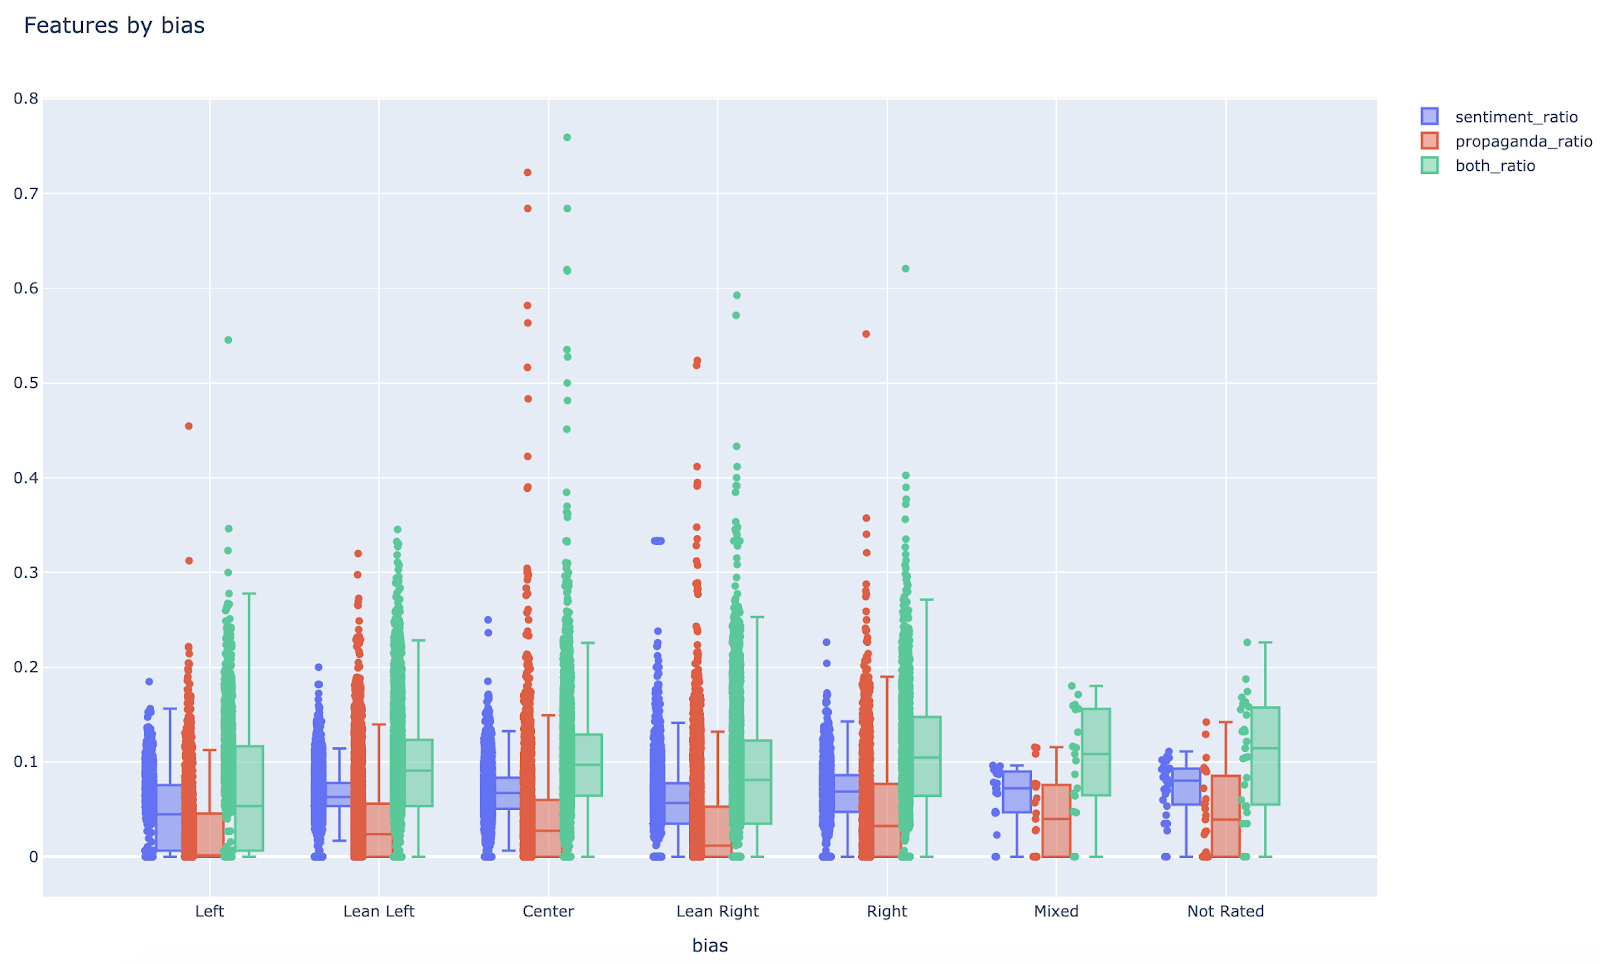
\includegraphics[width=\linewidth]{figures/4.3_prop_sent_across_leaning.png}
% %     \caption{Comparison of the detected sentiment and propaganda across the political leaning}
% %     \label{fig:prop_sent_across_leaning}
% % \end{figure}
% % \todo{Replace Figure~\ref{fig:prop_sent_across_leaning} with the one cleaned up, next in google docs}

% This plot in Figure~\ref{fig:prop_sent_across_leaning} is a quartile representation (with data points on the left of the boxes) which shows the distribution of the ratios computed. We can see that the average value (the line in the middle of the box) of “both\_ratio” is the highest for the “Right” side.
% From this plot we see that there are some very strange values (76\% of highlighted words in one article from the center). Looking at the details, this is an article from BBC which does not look so subjective. The problem is that from the full article, the scraping library only captured the sentence The statement says: ``It is an assault on UK sovereignty and any such use by a State party is a clear violation of the Chemical Weapons Convention and a breach of international law. It threatens the security of us all." which is annotated as almost everything propaganda. For other BBC articles, scraping manages to retrieve the full text without problems.

% There are also a lot of articles which have a percentage of 0\%. Looking at the distribution of the length of the documents, some documents, especially from some sources, have length=0 or a very short length (scraping the cookie disclaimer instead of the full article).
% For this reason a minimum length threshold has been set to cut out these problems: 150 tokens at least.

% This is the same plot, but with the filter on the minimum length.
% We can see that:
% The most annotated side is the Right
% The least annotated side is the Left
% Article from the Center do not contain less sentiment/propaganda (against assumption)
% There are less propaganda words than sentiment words



% 3. Creation of modified documents without the sentiment/propaganda parts
% As in the previous experiment (clustering), for each document other three documents have been created:
% Without propaganda words
% Without sentiment words
% Without propaganda and sentiment words
% Each document is embedded with two different methods:
% Universal Sentence Encoder
% TF-IDF (TODO dimensionality reduction, now it is a local TF-IDF to the cluster, see next point)


% 4. Comparing the articles about the same story
% Using the labels from AllSides, where articles are put together in groups of three items (usually one from the left, one from the center, one from the right), we compute the pairwise similarity matrix by using the embedded representations.
% For each cluster (provided by AllSides) we have 12 documents:
% Left-Full: the article from the left side, the full text
% Left-NoSent: the article from the left side, without sentiment words
% Left-NoProp: the article from the left side, without propaganda words
% Left-NoBoth: the article from the left side, without propaganda and sentiment words
% Center-Full: the article from the center side, the full text
% Center-NoSent: the article from the center side, without sentiment words
% Center-NoProp: the article from the center side, without propaganda words
% Center-NoBoth: the article from the center side, without propaganda and sentiment words
% Right-Full: the article from the right side, the full text
% Right-NoSent: the article from the right side, without sentiment words
% Right-NoProp: the article from the right side, without propaganda words
% Right-NoBoth: the article from the right side, without propaganda and sentiment words
% These articles are compared with a 12x12 matrix where the values are the similarity between the pair of docs.
% NOTE: at the moment, TF-IDF is computed locally to each cluster. I need to do the dimensionality reduction to be able to scale to more documents

% These similarities are then merged for all the AllSides clusters (being careful with the labels which can be different) and a final matrix is computed by doing an average of the matrices from the single clusters.
% The result is a 24x24 matrix (6 bias labels, not only left/center/right, multiplied with 4 variations of the same article).
% With this matrix it is possible to observe if, removing some parts of the articles, the similarity scores increase or decrease between different political sides.


% Results

% \todo{figures import}

% Observations:
% Within the rectangles on the main diagonal (yellow bright): comparison of the original articles with the modified ones generated from it:
% The removals are not changing the representations a lot: the scores are all quite high (minimum around 92% of similarity)
% The removal of propaganda parts is keeping the documents very similar to the original ones: average 98% similarity
% The removal of sentiment is changing a bit more the representation of the articles: minimum 93%, average 95%
% Increasing values between different biases (main diagonal of each block, see below):
% Usually similarity increases from Full article to noBoth
% Removing sentiment increases similarity (best scores)
% Removing propaganda decreases similarity a bit
% TODO: find a better way to represent this result. Just look at the main diagonals of each block, not so interesting to see the comparison between full articles and 

% Further improvements (TODOs):
% Propaganda/sentiment used by political sides by topic: break down by topic
% Propaganda types and sentiment scores by political sides: break down by fine-grained labels
% Verify correlation between propaganda:loaded\_language and sentiment. It is probably the same thing
% Improve visualisations of similarity changes (heatmap so big is confusing)
% Use dimensionality reduction and use a single TF-IDF model


% \todo{the rest (shapes...) goes in topic breakdown (next chapter)}


% Types of shapes (propaganda)
% (look at purple: propaganda)

% Blue is sentiment (+ and -) and purple is propaganda. 
% y axis in the fraction of terms marked as sentiment/propaganda.



\subsection{\statusorange Political leaning prediction using propaganda features}
\label{ssec:ps_prop_leaning_classifier}

% 5: political leaning classifier from propaganda features. Why
Here in this section, we take a different approach.
In the previous section, we saw how propaganda is slightly different considering the political leanings.
Here we take that result and we try to reverse the problem: using the features of propaganda extracted from the articles, can we automatically predict the leaning of the article?

This is what our RQ2 asks: \emph{Can we predict the political leaning of a news article by observing the propaganda it uses?}

Why the two could benefit / be related?

\todo{link here and avoid the repetition down from CIMPLE report}

The point of contact between political leaning prediction and propaganda is that both are dealing with political analysis.
Given that the facts that are being narrated are the same (exception: inclusion/exclusion), the main difference between an article from the left to one from the right is their point of view / subjective / persuasive component. Propaganda analysis is focused on analysing this specific component of the articles, the anti-topic model.
On this, we have our hypothesis that \emph{we can recognise the political leaning of an article by using the features provided by the propaganda analysis}.
The mixed analysis would allow to understand better why a certain article is classified as being left/right with respect to the black box BERT classifier.

The following sections first describe the general setup of the experiment, then deal with each one of the three research questions that we listed in the introduction: quantity, quantity by type, terms analysis.% TODO , context.


Unlike previous work on political leaning detection, in this experiment we use a propaganda detection method (from \citet{da2019fine}) to identify the existence of propaganda and its type of technique in given articles, and incorporate this information directly as additional features into the training and testing of the model.  


We also experimented briefly with sentiment features, but after seeing the null results (and also the results from the previous experiment), we decided not to proceed with sentiment but only with propaganda. Therefore from here we switch our terminology from \emph{persuasion} (propaganda+sentiment) to \emph{propaganda}.


% THIS IS FROM CIMPLE REPORT / TTO paper
In the experiment reported in this section, different types of propaganda used in news articles are used for identifying the political leaning of the articles. 
Propaganda is a regularly used technique in media and politics that aims to influence the perception of the audience and to sway their opinions in specific directions. However, it is unclear to what extent can we automatically identify the political leaning of news from their use of propaganda. This experiment investigates the use of propaganda features as input to an automated political leaning classifier.
Propaganda is usually directly linked to the ideology of articles by having the ``intention of influencing people’s opinions". To this end, we aim to better understand the relationship between propaganda analysis and the identification of political leaning of articles, simplified to three categories: Left, Centre, and Right.
Our hypothesis is that it is possible to recognise the political leaning of an article by using the features extracted through propaganda analysis. In other words, we hope to boost the performance of political leaning classifiers by learning which and how propaganda techniques are being used by which political side. This leads to three sub-research questions, aimed to see if it is possible to recognise the political leaning of articles from the:
Total amount of propaganda found in the text (RQ3.1)
Amount of each propaganda technique in the text (RQ3.2)
Specific words belonging to propaganda techniques in the article text (RQ3.3)
In this experiment, we use a propaganda detection method proposed in~\citet{da2019fine} to identify the existence of propaganda and its type of technique in given articles, and incorporate this information directly as additional features into the training and testing of the model.

\subsubsection{Dataset}
\todo{move to \ref{ssec:ps_leaning_classifier}}
The dataset used in this experiment~\citep{baly2020we} consists of articles in English language from over 800 sources (majority from the US), labelled for their political leaning (Left, Centre or Right). This dataset contains several attributes for each article: full text, political leaning, topic, news source, and author name. However, in our models and experiments, we only use the text of the articles to avoid bias associated with the other attributes. The topic distribution of the articles is uniform across the political leanings, because the dataset comes from triples of articles, one from each political leaning, about the same issue. The dataset contains two pre-split folds for training and testing:
Random: where splits are randomly generated. This classification model might encounter articles from the same media source during both training and testing phases.
Media: where the articles in the test set are from media sources that do not occur in the training set.

\subsubsection{Experimental Setup}

CIMPLE VERSION

The following steps are followed in this experiment:
 Implement the BERT-based political-leaning classifier described in~\citet{baly2020we} and apply it to the dataset to detect the political leaning of each article to reproduce the baseline results.
 Extract propaganda for each article using the tool from~\citet{da2019fine}.
Add propaganda-related features to the BERT model, by injecting the values in the neural network using the (a) total presence of propaganda as a feature (Experiment 1), (b) percentage of each propaganda technique (Experiment 2), and (c) words that appear in the detected propaganda text (Experiment 3).
Train and test the model under different configurations with two splits, one   one less biased to media source.
Compare our results with two baselines; the majority class (where the political leaning is assumed to be that of the most popular leaning in the dataset), and the results from our re-implementation of the model in step 1

TTO2019 VERSION
% General things before experiments
Our experiments are designed to test the role of propaganda features in detecting the political leaning of articles. The following steps are followed in our experiments:
\begin{enumerate}
 %   \item ... ?collect data from AllSides ...
    \item Implement the BERT-based political-leaning classifier described in~\citet{baly2020we} and apply it to the dataset to detect the political leaning of each article to reproduce the baseline results.
    \item Extract propaganda for each article using the tool from~\citet{da2019fine}.
    \item Add propaganda-related features to the BERT model, by injecting the values in the neural network using the (a) total presence of propaganda as a feature (Experiment 1), (b) percentage of each propaganda technique (Experiment 2), and (c) words that appear in the detected propaganda text (Experiment 3).
    \item Train and test the model under different configurations with two splits, one totally random, and one less biased to media source.
    \item Compare our results with two baselines; the majority class (where the political leaning is assumed to be that of the most popular leaning in the dataset), and the results from our re-implementation of the model in step 1. %of \cite{baly2020we}.
\end{enumerate}

\paragraph{Political Leaning Model}
Our baseline is the same as described in the previous Section~\ref{ssec:ps_leaning_classifier}.

\todo{figure with network}


\paragraph{Propaganda Features}

CIMPLE VERSION

The extraction tool~\citep{da2019fine} extracts 18 propaganda techniques (listed in Figure 5). We apply this tool to the articles in our dataset to obtain these propaganda annotations. We use these annotations to calculate several numerical features that we employ in the following three sections to answer the three research questions.
Our analysis workflow is depicted in Figure 6. Each article in the dataset is passed through the baseline BERT pre-trained models to calculate the baseline result, and through our models that incorporate the various propaganda features to calculate the results from our three experiments.
We calculate the F1-macro and accuracy of the models and compare them with each other and with the baseline. We also evaluate the significance of each added feature from the weight assigned to them by the classification model (the higher the weight, the more discriminative the feature is for Left/Centre/Right-leaning articles). We also combine the features given by each feature set, to see whether the addition of certain features helps to achieve higher classification accuracy. This combination is performed by concatenating the inputs to the SoftMax dense layer. It is not a combination of trained models, but it is a model that is trained and used on a combination of input features.


TTO2019 VERSION

As mentioned earlier, for the propaganda analysis, we use the state of the art approach provided in~\citet{da2019fine}.\footnote{\url{https://huggingface.co/QCRI/PropagandaTechniquesAnalysis-en-BERT}} Their tool extracts 18 propaganda techniques. We apply this tool to the articles in our dataset to obtain these propaganda annotations. 
%and we gather the annotation for the articles in the dataset by using the official model released.
%API.\footnote{\url{https://app.swaggerhub.com/apis-docs/yifan2019/Tanbih/}}
%This model provides as result a set of spans from the text with a label corresponding to one of the 18 techniques.
% In addition to the propaganda techniques, we also run lexicon-based sentiment analysers to obtain a set of words loaded with sentiment with their polarity value (positive vs negative).
We use these annotations to calculate several numerical features that we employ in the following three sections to answer the three research questions introduced in Section \ref{sec:intro}.
%\begin{enumerate}
 %   \item the total quantity of propaganda (first
 %   \item the quantity of each propaganda technique
 %   \item the frequency of words that have been annotated for each propaganda technique
%\end{enumerate}

% The extracted features are then fed to a classifier that can be \sout{a SVM or} a Neural Network (single dense layer with softmax activation function).
% The train/test split for the 13k and 60k datasets is done with stratified split (to keep the proportion of L/C/R in the two splits): 90\% train, 10\% test.


Our analysis workflow %model architecture we use 
is depicted in Figure~\ref{fig:model_classifier}. Each article in the dataset is passed through the baseline BERT pre-trained models to calculate the baseline result, and through our models that incorporate the various propaganda features to calculate the results from our three experiments. %\todo{correct?} 
%Each article in the dataset is passed through either the baseline BERT pre-trained models, or the models that incorporate the various propaganda features. 
%The model The orange parts are being trained with the training set: the final SoftMax layer and the term-frequency analysis.

\begin{figure}[!htb]
    \centering
    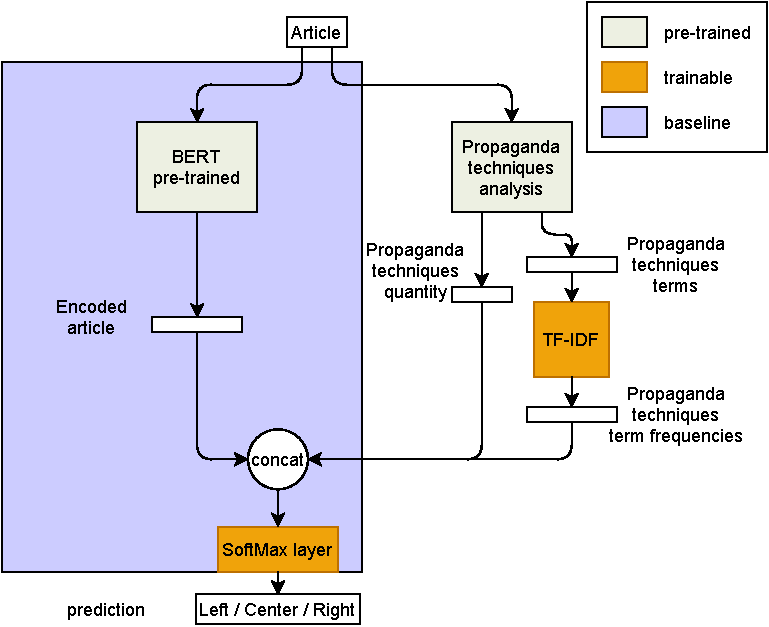
\includegraphics[width=\linewidth]{figures/methodology-Page-1.pdf}
    \caption{The model architecture. Baseline model on the left. On the right are our propaganda-based models.}
    \label{fig:model_classifier}
\end{figure}

We calculate the F1-macro and accuracy of the models and compare them with each other and with the baseline. % in search of any changes and improvements.%  we try to understand if there are some improvements for each of the three sections, and what is their statistical significance.
We also evaluate the significance of each added feature from the weight assigned to them %to each features 
by the classification model (the higher the weight, the more discriminative the feature is for Left/Centre/Right-leaning articles). %by looking at the weights of the models used, to understand what they learned.

%In some cases, 
We also combine the features given by each feature set, to see whether the addition of certain features helps to achieve higher classification accuracy. %values for the metrics. 
This combination is performed by concatenating the inputs to the SoftMax dense layer. It is not a combination of trained models, but it is a model that is trained and used on a combination of input features.


\subsubsection{Total Quantity of Propaganda}


\begin{table}[!htbp]
    \centering
   \scriptsize
  %\small
    % \resizebox{\textwidth}{!}{
    \begin{tabular}{l|rr|rr}
        & \multicolumn{2}{c}{Random} & \multicolumn{2}{c}{Media} \\
        Model & F1-Macro & Accuracy & F1-Macro & Accuracy \\
        \hline
        \texttt{Majority} & 21.0286 & 46.0769 & 21.0286 & 46.0769 \\
        % \texttt{Baly-API} & 42.3355 & 43.8356 & 42.0523 & 43.6910 & 41.6863 & 41.7993 & & & & \\
        \texttt{Baly-baseline} (0) & \textbf{56.4447} & \textbf{58.6153} & 40.8647 & 46.2307 \\
        %\texttt{Baly-paper} (*) & 80.19 & 79.83 & 35.53 & 36.75 \\
        \hline
        \texttt{Prop-Total} (1) & 36.2966 & 42.3076 & 28.8285 & 41.5384 \\
        \texttt{Prop-Techniques} (2) & 36.7166 & 40.6153 & 33.0682 & 40.5384 \\
        \texttt{Prop-Total-Terms} (3a) & 42.0261 & 43.5384 & 41.5915 & 43.3076 \\
        \texttt{Prop-Techniques-Terms} (3b) & 42.4357 & 43.2307 & 40.8192 & 41.9230 \\
        % \texttt{Prop-words-BERT} (3) & 35.4718 & 48.2387 & 35.4718 & 48.2387 \\
        \hline
        (0) + (1) & 55.7786 & 57.7692 & 42.1847 & 47.5384 \\
        (0) + (2) & 54.9714 & 56.9999 & 42.4362 & \textbf{47.6153} \\
        (1) + (2) & 36.5217 & 40.4615 & 33.6202 & 41.0000 \\
        (0) + (1) + (2) & 55.2121 & 57.1538 & 42.2102 & 47.3846 \\
        (0) + (3a) & 54.6287 & 56.6923 & 41.9766 & 46.5384 \\
        (0) + (3b) & 54.8004 & 56.3076 & 41.9965 & 46.2307 \\
        (3a) + (3b) & 44.3506 & 46.3076 & 41.8725 & 44.3076 \\
        (0) + (3a) + (3b) & 53.2549 & 54.7692 & 42.0576 & 45.92307 \\
        (1) + (2) + (3a) & 42.0611 & 43.8461 & 42.5401 & 44.5384 \\
        (0) + (1) + (2) + (3a) & 54.0515 & 56.0769 & 42.2358 & 46.8461 \\
        (1) + (2) + (3b) & 44.3166 & 45.6153 & 41.9613 & 44.0000 \\
        (0) + (1) + (2) + (3b) & 45.6153 & 45.6153 & 41.9292 & 46.2307 \\
        (1) + (2) + (3a) + (3b) & 45.0456 & 47.2307 & \textbf{43.4564} & 45.9230 \\
        (0) + (1) + (2) + (3a) + (3b) & 53.6459 & 53.6459 & 42.5509 & 46.5384 \\
        
    \end{tabular}
    % }
    \caption{Results given by the different features. Baselines above, RQ3.1=\texttt{Prop-Total}, RQ3.2=\texttt{Prop-Techniques}, RQ3.3= (\texttt{Prop-Total-Terms} and \texttt{Prop-Techniques-Terms}). The last group shows various combinations of features that in some cases provide improvements over the baseline.}
    \label{tab:results_prop_features_classifier}
\end{table}

CIMPLE VERSION

Considering only the total amount of propaganda in each article, we calculate a single value to represent the percentage of propaganda text inside the article (i.e., the ratio between the number of propagandist words and the total number of words) to answer RQ1.
Figure 7 shows how this value is distributed across Left, Centre and Right leaning articles. Table 6 shows the results of this first experiment under the name Prop-Total. The low values, just above the Majority baseline, indicate that the feature is unsuitable for determining which side an article belongs to. Both F1 and accuracy are below the values of Baly-baseline for both Random and Media splits. Thus, the answer to RQ1 is No, the total amount of propaganda in an article does not seem to be a good indicator of the political leaning of an article.

TTO2019 VERSION
Our hypothesis behind RQ1 is that the total quantity of propaganda contained in an article helps to recognise its political leaning. 
% definition
To answer RQ1, we consider only the total amount of propaganda detected in each article. For each article, we calculate a single value to represent the percentage of propaganda text inside the article. %Using a percentage compensates for the varying lengths of articles.%These words are the one annotated as propaganda by \cite{da2019fine} (see Section \ref{sec:prop}).
% how it is computed
We use a percentage in order to be less biased and independent of the article size.
This value is computed for each article as the ratio between the number of words detected as propagandist (see Section \ref{sec:prop}) and the total number of words. For example, if an article has 600 words, and propaganda analysis annotated 30 of them as being propagandist, the value of the feature will be 5\%.  
% hypothesis
%The hypothesis is that by observing the total quantity of propaganda contained in an article, we can recognise its political leaning.
% stats
As we saw in the previous Section~\ref{ssec:ps_prop_leaning_across} in Figure~\ref{fig:prop_sent_across_leaning}, the distributions of the total quantity of propaganda was quite similar, but it has lower values in the Center and higher values in the Right.
%Figure~\ref{fig:tot_quantity} shows how this value is distributed across Left, Centre and Right leaning articles. It appears that all three groups have a similar propaganda distribution. The Centre appears to have slightly less propaganda, and the Right sources have the most (could be due to propaganda bias as we highlight later in Section~\ref{sec:discussion}).%, especially looking at the dots that represent the outliers. 
% TODO better figure
 %Overall, the boxplot shows that the presence of propaganda is similar across the board.%, and the results in Table \ref{tab:results_rq123} show that adding this feature lowers our classification accuracy. Hence %mostly overlap so this is a negative sign for our hypothesis.
%the answer to RQ1 is No, the mere presence of propaganda is insufficient to determining the political leaning of articles. 

% TODO: rename categories in plot to L/C/R
% \begin{figure}[!htb]
%     \centering
%     \includegraphics[width=\columnwidth]{figures/total_prop_data_condensed_mod.jpg}
%     \caption{Boxplot of the total amount of propaganda in Left, Centre and Right articles.}
%     \label{fig:tot_quantity}
% \end{figure}

% TODO move baseline considerations to section 3? When model will be shared by baly, this won't exist anymore
% Table~\ref{tab:results_rq123} contains in the first group the baselines considered:

% \begin{itemize}
%     \item The \texttt{Majority} baseline, just providing the most common class as output, has quite low results and is considered here just as lower threshold on the other values.
%     \item \texttt{Baly-baseline}, being an emulation of what described in~\citet{baly2020we}, is still far from the 80\% results reported by the authors. For sure the source-code sharing from them that we are waiting will make the results improve
%     % \item \texttt{Baly-API} instead has much lower results that \texttt{Baly-baseline}, and therefore we can conclude that it is definitely not the implementation of the model described in~\citet{baly2020we}. It is coming from the same research group but we need to ask to the maintainers which results is it providing.
% \end{itemize}

Table~\ref{tab:results_rq123} shows the results of this first experiment under the name \texttt{Prop-Total}. The low values, just above the \texttt{Majority} baseline, indicate that the feature is unsuitable for determining which side an article belongs to. Both F1 and accuracy are below the values of \texttt{Baly-baseline} for both Random and Media splits. Even combining this feature with the baseline (i.e. adding propaganda percentage as features to the BERT model) does not provide an improvement, as shown by the row denoted by (0) + (1).



% % confusion matrix
% Looking at the confusion matrix of the 60k dataset in Figure~\ref{fig:total_prop_confusion_60k}, we can see that the model learned to predict the class with most articles, with a few exceptions that are classified as Right (probably the articles with a lot of propagandistic content, TODO compare with learned weights). A similar result can be seen in the 13k dataset. If instead we look at the balanced dataset, Figure~\ref{fig:total_prop_confusion_60k_balanced}, the models shifts to predicting random labels between Centre and Right.
% This means that, removing the shortcut~\cite{geirhos2020shortcut} of ``everything belongs to the Left'', the model cannot pick any relevant information from the feature described above.
% For the \texttt{baly} dataset instead,
The confusion matrix in Figure~\ref{fig:total_prop_confusion} shows that the classifier is introducing biased predictions towards the Right-leaning class. %From observing that in general right-leaning articles contain more propaganda overall (\texttt{Prop-Total} feature), the results are skewed right. 
This results in higher recall but lower precision for the Right class, and almost zero accuracy for the Centre label. 

In summary, the answer to RQ1 is \textbf{No, the total amount of propaganda in an article does not seem to be a good indicator of the political leaning of an article}.

% provides a low result overall but a quite good F1 on the Right class.

% \begin{figure}[!h]
%     \centering
%      \begin{subfigure}[b]{0.45\linewidth}
%          \centering
%          \includegraphics[width=\linewidth]{figures/nodes_stratified_confusion_matrix_propaganda_total_percentage.pdf}
%          \caption{Unbalanced 60k}
%          \label{fig:total_prop_confusion_60k}
%      \end{subfigure}
%     %  \hfill
%     \begin{subfigure}[b]{0.45\linewidth}
%          \centering
%          \includegraphics[width=\linewidth]{figures/nodes_stratifiedbalanced_confusion_matrix_propaganda_total_percentage.pdf}
%          \caption{Balanced 60k}
%          \label{fig:total_prop_confusion_60k_balanced}
%      \end{subfigure}
%      \\
%      \begin{subfigure}[b]{0.45\linewidth}
%          \centering
%          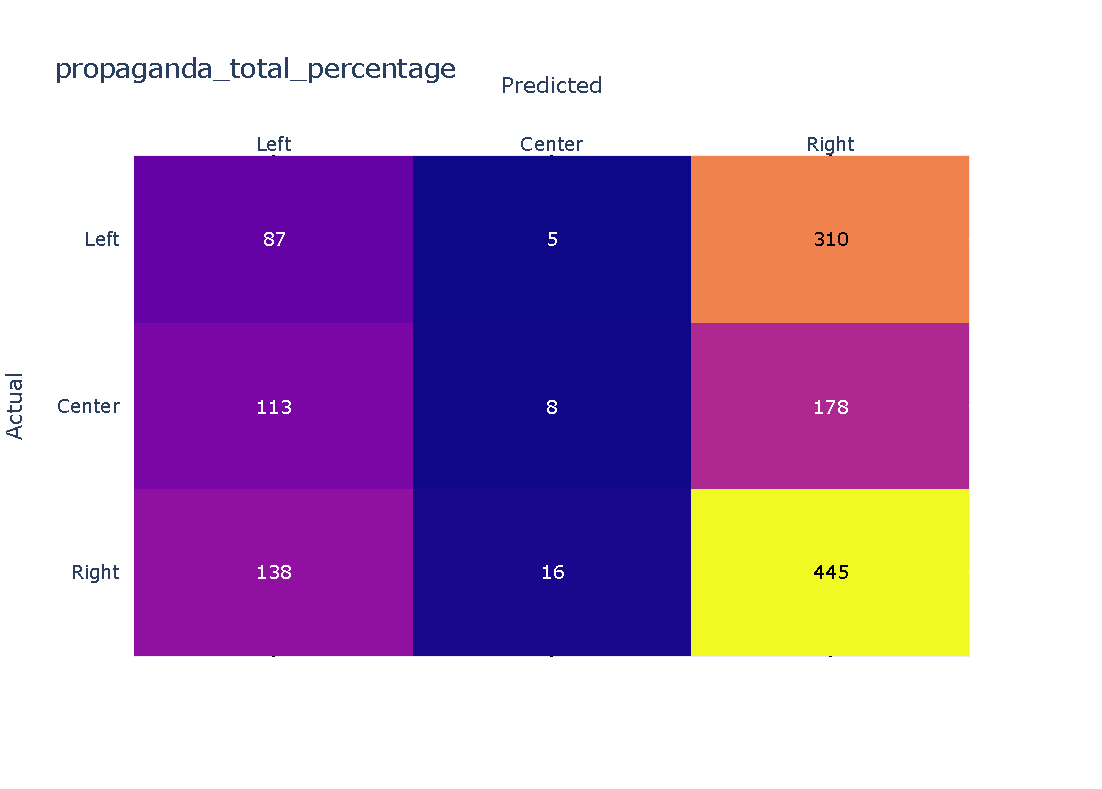
\includegraphics[width=\linewidth]{figures/baly_media_confusion_matrix_propaganda_total_percentage.pdf}
%          \caption{Baly}
%          \label{fig:total_prop_confusion_baly}
%      \end{subfigure}
%     \caption{Confusion matrix of the classifier using the features of \texttt{Prop-Total}.}
%     \label{fig:total_prop_confusion}
% \end{figure}

\begin{figure}[!htbp]
    \centering
    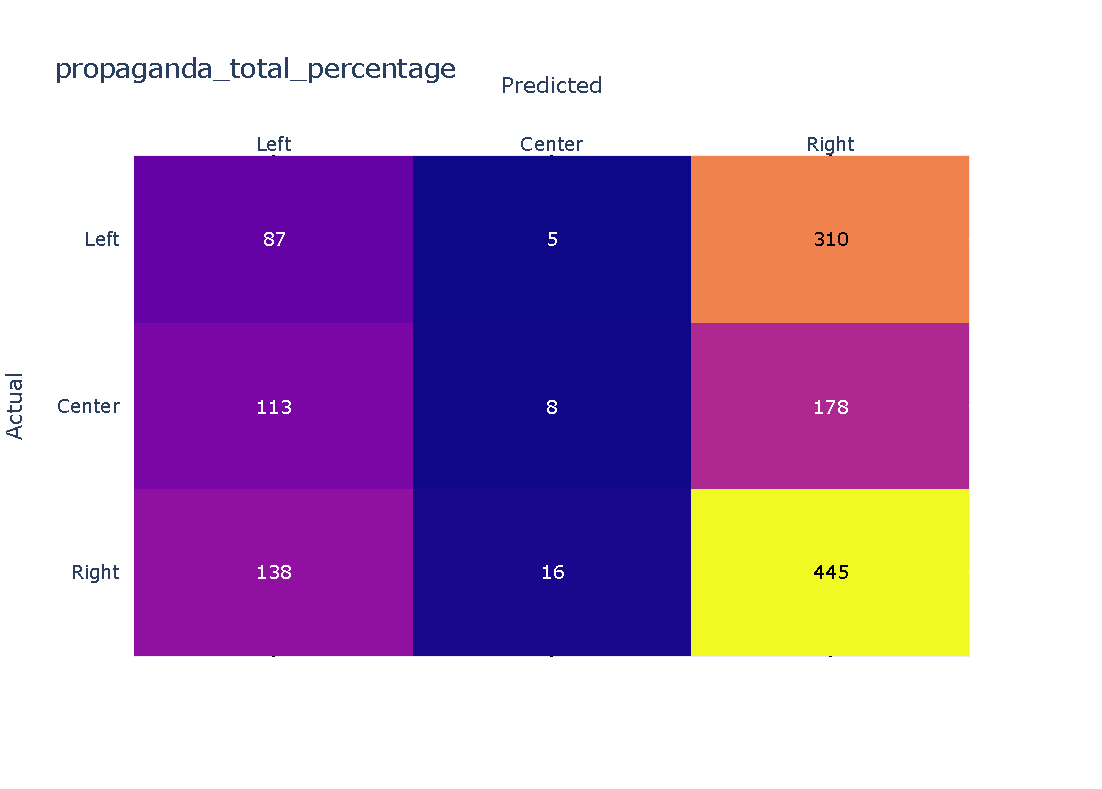
\includegraphics[width=0.75\linewidth]{figures/baly_media_confusion_matrix_propaganda_total_percentage.pdf}
    %\vspace{-1cm}
    \caption{Confusion matrix of the classifier using the \texttt{Prop-Total} features (RQ1).}
    \label{fig:total_prop_confusion}
\end{figure}

% TODO: double-check: if we explained the reasons for the classifier, inspecting the weights does not make sense
% % what the model learned:weights
% If we inspect the weights learned by the model in figure~\ref{fig:total_prop_weights}, the network simply learned that propaganda is mostly associated with the Left and not with the Center; the left is in the middle.
% This works well for the left-leaning articles (only 247 out of 2499 are mis-classified) while it does not produce good results for the other two political leanings.
% The decision based only on this feature acts in the following way:
% \begin{itemize}
%     \item if an article has low quantities of propaganda, it is put in the Left bucket (almost all the articles)
%     \item if an article has high quantities of propaganda, it is put in the Right bucket
%     \item no articles are put in the Center bucket (they should have negative quantities, according to the weights)
% \end{itemize}

% \begin{figure}[!h]
%     \centering
%     \includegraphics[width=\linewidth]{figures/total_prop_weights.png}
%     \caption{Weights of the classifier using only the total propaganda quantity: yellow means positive signal and purple means negative signal.}
%     \label{fig:total_prop_weights}
% \end{figure}

% significance

% The last row of Table~\ref{tab:q_60k} presents the combination of this feature with the baseline, which results in a small degradation of the baseline. This feature is not enough to recognise political leaning.


\subsubsection{Quantity of Propaganda Techniques}

CIMPLE VERSION

Testing the role of the presence of particular propaganda techniques in determining the political-leaning, RQ2, compute the word-based percentage of each technique inside each article and used the features obtained to classify articles. The value for each technique is equal to the number of words belonging to it, divided by the total number of words in the document.
We train the classifiers as the in previous experiment and obtain the result indicated by Prop-Techniques (2) in Table 6. Although the results show improvement over the previous experiment, they are still well below the best performing baseline. The results show that (a) Prop-Techniques alone is insufficient to accurately detect the political leaning of articles (RQ2), and (b) when Prop-Techniques is added to Baly-baseline (line (0) + (2) in results table), it brings an improvement on the Media split for both the F1 and accuracy measures. 
Given the improvements in some cases, we perform an additional test to better understand the significance of these results. To perform this test, we build a contingency table by considering two arrays: the first shows when the Baly-baseline produced the correct result on the test set, and the second one shows when the line (0) + (2) (baseline+propaganda techniques quantity) produced the correct result on the Media split. The contingency table, therefore, is a 2x2 matrix.
Using the predicted labels of the selected rows on the Media split (last two columns of Table 6), the (0)+(2) against baseline resulted in a pvalue=0:008, which means that the improvement is significant. Remember that the Media split is less biased than the Random split, since in the Media split the sources of the articles in the test set are not overlapping with the sources of the articles in the training set. If we compare the Random vs Media split results, we can see that while the Baly-baseline drops significantly (more than 15\% F1 and 12\% accuracy), the models based on the features of propaganda have a much smaller drop in these measures (less than 8\% F1 and less than 1\% accuracy). This means that our models with propaganda features are coping better with articles from “new sources” that are unseen in the training set. The improved generalisation abilities of this feature are perhaps what is driving the significant improvement described above.
The conclusion of this experiment is that the amount of each propaganda technique is not enough on its own to accurately recognise the political leaning of an article, but when combined with the baseline features produces a significant improvement.

TTO2019 VERSION

In this section, we test the hypothesis of RQ2, which is that the presence of particular propaganda techniques helps to determine the political-leaning of articles. 

%From the negative results to the first research question, we make another step to use more detailed features. 
Instead of relying on a single value of total propaganda quantity as in the previous experiment, we now consider the amount of each propaganda technique to train the political-leaning classifier.
% The second step we take is to break the quantities of propaganda with respect of each one of the techniques.
The motivation behind is that a specific political leaning (e.g. Right-leaning) may be using one or more techniques more than others, and the classifier could pick these differences to perform its decisions.
This means that our feature vector is not a one-value vector but instead it is an 18-values vector, each one representing the amount of a specific propaganda technique (See Section \ref{sec:prop}).


We compute the word-based percentage of each technique inside each article. This means that the value for each technique is equal to the number of words belonging to it, divided by the total number of words in the document. A value of 1\% means that 1 out of 100 words in the document have been spotted as being part of the considered propaganda technique.
%We use a percentage, as in the previous case, in order to be independent on the article size.

% TODO: too small and messy figure
% \begin{figure}[!htb]
%     \centering
%     \includegraphics[width=\columnwidth]{figures/baly_prop_techniques_together.pdf}
%     \caption{Distribution of the amount of propaganda techniques in our dataset across Left (blue), Centre (green), and Right (red).}
%     \label{fig:prop_perc}
% \end{figure}

% data distribution
%To give an idea of the computed percentages, we grouped the articles according to their political leaning \textcolor{red}{as determined by AllSides}. 
As we have seen in the previous Section~\ref{ssec:ps_prop_leaning_across},  Figure~\ref{fig:prop_tech_details_across_leaning} was showing that the amount of propaganda techniques detected in these groups of articles is generally low. The most prominent one is the \texttt{Loaded\_Language}.
As in the previous subsection, we observe that articles from the Centre appear to be using fewer propaganda techniques, %, while Left and Right have higher percentages. This is expected given the overall propaganda use pattern found in the previous experiment.   %However, the difference seems minimal overall. 
but as we noted, there are some techniques which have different shapes (U-shape, triangular shape). Our hope is that an automated classifier is able to pick these different patterns and use them to differentiate the political leaning. 


% A similar procedure has been done for the sentiment analysis. First, sentiment words have been extracted by several lexicons (TODO list). In this way every sentiment-loaded term in the articles analysed is associated with its polarity value (positive or negative).
% Then with these annotations we extracted the percentage of positive tokens and negative tokens and used these as input features.




% - Classifier with features: results and significance
We train the classifiers as the in previous experiment and obtain the result indicated by \texttt{Prop-Techniques} (2) in Table~\ref{tab:results_rq123}. Although the results show improvement over the previous experiment, they are still well below the best performing baseline. %This indicates that 
%As for the previous case, we have generally low scores, slightly improved from RQ1 on both splits.
The results show that (a) \texttt{Prop-Techniques} alone is insufficient to accurately detect the political leaning of articles (RQ2), and (b) when \texttt{Prop-Techniques} is added to \texttt{Baly-baseline} (line (0) + (2) in results table), it brings an improvement on the Media split for both the F1 and accuracy measures. 


%\begin{enumerate}
%    \item \texttt{Prop-Techniques} alone does not provide good results;
%    \item When \texttt{Prop-Techniques} is added to \texttt{Baly-baseline} in line (0) + (2), it does bring an improvement on the media split for both the F1 and accuracy measures.%, which is even bigger when added to the feature from the previous section.
    % \item When \texttt{Prop-Techniques} is added to \texttt{Baly-baseline} on the \texttt{Baly} dataset, it has a big improvement on both F1 and Accuracy
%\end{enumerate}

Given the improvements in some cases, we perform an additional test following the approach in~\citet{mcnemar1947note} 
to better understand the significance of these results. %if this is just a small effect or if it is something significant.
To perform this test, we build a contingency table by considering two arrays: the first shows when the \texttt{Baly-baseline} produced the correct result on the test set, and the second one shows when the line (0) + (2) (baseline+propaganda techniques quantity) produced the correct result on the Media split. The contingency table, therefore, is a 2x2 matrix as shown in 
% Table~\ref{tab:contingency} and 
Table~\ref{tab:contingency2}.

% \begin{table}[]
%     \centering
%     \begin{tabular}{c|c|c}
%         & \multicolumn{2}{c}{(0)+(1)+(2)} \\
%          & incorrect & correct \\
%          \hline
%         (0) incorrect & 2013 & 91 \\
%         (0) correct & 75 & 3868
%     \end{tabular}
%     \caption{Contingency table for 60k}
%     \label{tab:contingency}
% \end{table}

\begin{table}[]
    \centering
%    \scriptsize
\small
    \begin{tabular}{c|c|c}
        & \multicolumn{2}{c}{(0)+(2)} \\
         & incorrect & correct \\
         \hline
        (0) incorrect & 672 & 27 \\
        (0) correct & 10 & 591
    \end{tabular}
    \caption{Contingency table on Media splits.}
    \label{tab:contingency2}
\end{table}


% The first addition, when tested for significance with McNemar test with respect to the baseline, it provided a p-value=0.244 for 60k and p-value=0.608 for 13k. The values means that the contribution is not significant.
% Looking at the values of the contingency table, we can see that for the 60k dataset, adding the features from (1) and (2) made 91 elements of the test set to be correctly classified (misclassified instead from the baseline), but at the same time it brought other 75 elements with a correct label according to the baseline to be incorrectly classified.

% TODO move this in a more visible section, like final discussion? This applies to all the propaganda features
Using the predicted labels of the selected rows on the Media split (last two columns of Table~\ref{tab:results_rq123}), the \texttt{(0)+(2)} against baseline resulted in a \textbf{p-value=$0.008$}, which means that the \textbf{improvement is significant}.
Remember that the \textbf{Media split is less biased than the Random split}, since in the Media split the sources of the articles in the test set are not overlapping with the sources of the articles in the training set. If we compare the Random vs Media split results, we can see that while the \texttt{Baly-baseline} drops significantly (more than 15\% F1 and 12\% accuracy), the models based on the features of propaganda have a much smaller drop in these measures (less than 8\% F1 and less than 1\% accuracy).
This means that our models with propaganda features are coping better with articles from ``new sources'' that are unseen in the training set. 
The improved generalisation abilities of this feature is perhaps what is driving the significant improvement described above. %can be seen when put in combination with the features of the baseline with the significant improvement described just above \textcolor{red}{(sentence unclear)}. 


% confusion matrix
Figure~\ref{fig:prop_tech_confusion} is the confusion matrix for the classifier using the \texttt{Prop-Techniques} feature alone. It shows that the situation is very similar to the previous experiment. More articles are predicted as being Right-leaning with respect to the other two classes. %, because it is the most represented class.
% From the unbalanced situation in \ref{fig:prop_tech_confusion_60k}, where the articles were generally predicted to be Left leaning, the subfigure \ref{fig:prop_tech_confusion_60k_balanced} shows that after the correction most of the articles are classified on the Centre.
If we compare the subfigures~\ref{fig:prop_tech_confusion_baly_random} and~\ref{fig:prop_tech_confusion_baly_media}, we see that they are quite similar (F1 and accuracy are very similar too). The only difference is that the Media split predictions are a bit more Right-leaning biased, resulting in lower local F1 for Left and Centre.

\begin{figure}[!htb]
    \centering
    %  \begin{subfigure}[b]{0.45\linewidth}
    %      \centering
    %      \includegraphics[width=\linewidth]{figures/nodes_stratified_confusion_matrix_propaganda_percentages.pdf}
    %      \caption{Unbalanced 60k}
    %      \label{fig:prop_tech_confusion_60k}
    %  \end{subfigure}
    % %  \hfill
    % \begin{subfigure}[b]{0.45\linewidth}
    %      \centering 
    %      \includegraphics[width=\linewidth]{figures/nodes_stratifiedbalanced_confusion_matrix_propaganda_percentages.pdf}
    %      \caption{Balanced 60k}
    %      \label{fig:prop_tech_confusion_60k_balanced}
    %  \end{subfigure}
     \begin{subfigure}[b]{0.48\linewidth}
         \centering
         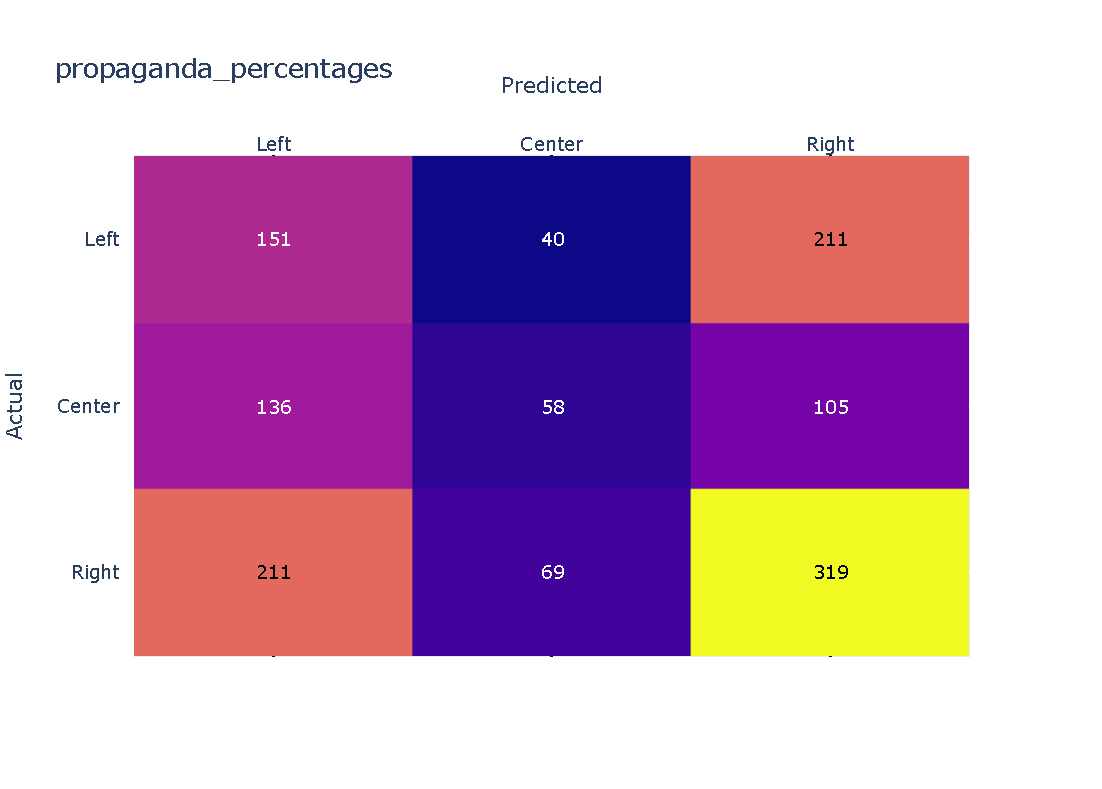
\includegraphics[width=\linewidth]{figures/baly_random_confusion_matrix_propaganda_percentages-small.pdf}
         \caption{Baly random}
         \label{fig:prop_tech_confusion_baly_random}
     \end{subfigure}
    %  \hfill
    \begin{subfigure}[b]{0.48\linewidth}
         \centering 
         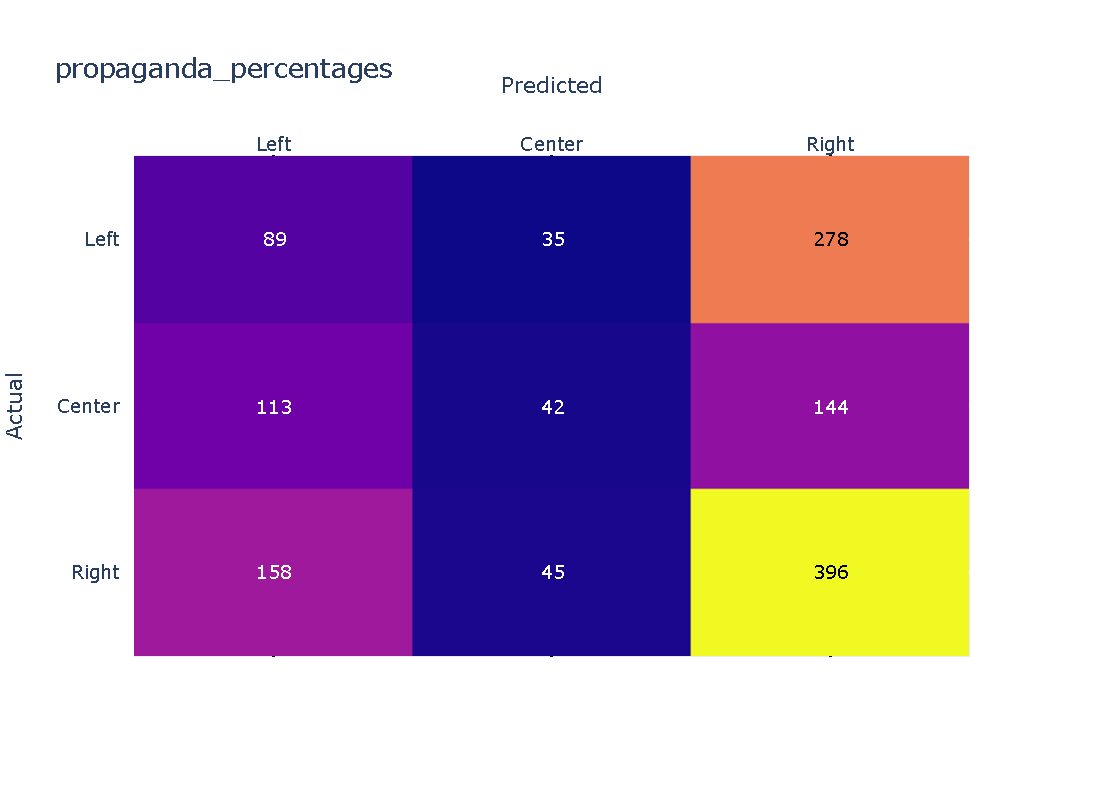
\includegraphics[width=\linewidth]{figures/baly_media_confusion_matrix_propaganda_percentages-small.pdf}
         \caption{Baly media}
         \label{fig:prop_tech_confusion_baly_media}
     \end{subfigure}
    \caption{Confusion matrix of the classifier using the features of \texttt{Prop-Techniques} (RQ2).}
    \label{fig:prop_tech_confusion}
\end{figure}

% features learned
To understand what the model has learnt, we investigate the weights assigned by the neural layer part of the model. We can see in Figure~\ref{fig:prop_tech_weights} that Right is associated with some propaganda techniques (e.g. Slogans and Reductio ad Hitlerum), while the Left is more associated with other techniques (e.g. Exaggeration/Minimisation and Name-Calling/Labeling).\footnote{For more information on each of these propaganda techniques, please refer to \cite{da2019fine}} The Centre is generally associated by the model with an absence of all  propaganda techniques. It is important to note that given the low F1 score of 40\%, the weight assigned by this model for each propaganda technique feature is only indicative. %does not not represent the ground-truth. 

%We need to specify that the weights observed do not directly represent the amount of each technique in the corpus. They represent only values that the neural layer assigned as internal weights to optimise the loss on the training set. If the models were having very nice performances we could say that what the model learned is correct, while in this case with values of F1 around 40\% the features learned do not represent quite well the political leaning.

\begin{figure}[!htb]
    \centering
    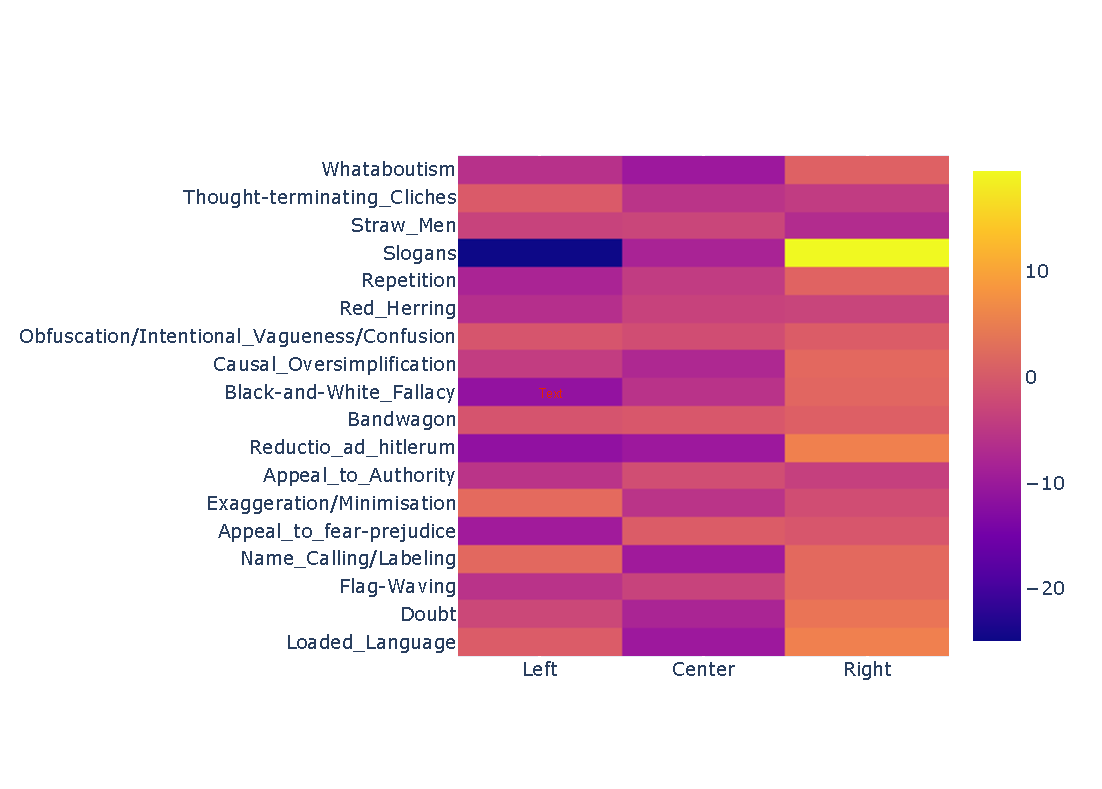
\includegraphics[width=\linewidth]{figures/nodes_stratifiedbalanced_weights_propaganda_percentages-small.pdf}
    \caption{Weights for \texttt{Prop-Techniques} on the balanced dataset: yellow means a positive signal, and purple means a negative signal.}
    \label{fig:prop_tech_weights}
\end{figure}

The conclusion of this experiment is that \textbf{the amount of each propaganda technique is not enough on its own to accurately recognise the political leaning of an article, but when combined with the baseline features produces a significant improvement}.


\subsubsection{Terms of Propaganda}

CIMPLE VERSION

To investigate the chosen terminology for expressing the identified propaganda techniques in articles for each political leaning (RQ3), the terms were analysed in two different ways:
(3a) all the propaganda words taken together: non-propaganda annotated words are filtered out. The classifier will then use the remaining propaganda words to learn any differences between political leanings.
(3b) propaganda words grouped by propaganda technique: there are 18 groups, one for each propaganda technique. The classifier will use the words, grouped by the technique to which they belong, to recognise the political leaning.
To obtain the feature vectors of the propaganda words, we use TF-IDF because its numerical values directly represent single terms. Instead with other embedding methods  this correspondence with single terms would be more difficult to extract. By considering the features which get assigned the biggest values in the final SoftMax layer, we can directly say which terms are the most discriminative for the task of political leaning classification. 
The row of Table 6with the label Prop-Total-Terms (3a) refers to the TF-IDF features computed by only using the propaganda terms, without differentiating between the different techniques. This row has significantly better results than (1) and (2) on both splits, but only outperform the Baly-baseline on the Media split in F1.
On the other hand, the feature Prop-Techniques-Terms (3b) refers to splitting the propaganda terms into the 18 groups and then computing the TF-IDF features on each group separately. The results of this feature set are generally a few decimal points below (3a).
With the current analysis, we can say that the answer to RQ3 is a partial Yes: using as feature the terms of propaganda achieves a very similar score to the baseline (rows indicated with (3a) and (3b)), and when added to the baseline features, it helps to achieve a small (but not significant, p-value=0.657) improvement.


TTO2019 VERSION

% TODO: keep together propaganda spans instead of tokenizing (e.g., "")
%Given the results of the two previous experiments, and the room for improvement that is left above the scores shown, we want to have a better understanding of the differences between the propaganda coming from multiple political sides.
Following on from the previous two experiments, we now aim to reach a better understanding of the differences between how propaganda is portrayed in articles belonging to each political side.
We need to go beyond the quantification of detected propaganda techniques (previous experiment), and investigate the chosen terminology for expressing these propaganda techniques in articles belonging to Left, Right, or Centre (RQ3). %how the techniques differ across the political spectrum with regards to used language. 
% to recognise political leaning given by the previous sections, the idea is to take a look at the specific terms picked up by the propaganda analysis. Not only quantity, but which words belong to each technique.

%To this end, the RQ3 considers as features the terms that are picked as part of the propaganda techniques.
The hypothesis is that, even though propaganda techniques are used with similar percentages (as learnt from the first two experiments), the choice of words and their frequency differ between different-leaning articles, which can improve their classification. 
%there are some specific words that are used by opposing leanings that are used with different frequency.


In this third experiment, we proceed with the analysis of terms in two different ways:
\begin{itemize}
    \item (3a) all the propaganda words taken together: non-propaganda annotated words are filtered out. The classifier will then use the remaining propaganda words to learn any differences between political leanings. 
    %this acts as an attention mask between the classifier and the articles, filtering out the words that are not propagandist. The classifier will then use the propaganda words to learn any difference between political leanings. 
    \item (3b) propaganda words grouped by propaganda technique: there are 18 groups, one for each propaganda technique. The classifier will use the words, grouped by the technique to which they belong, to recognise the political leaning.
\end{itemize}

While the objective of (3a) is to learn distinctive propaganda terms, (3b) instead focuses on the terms of the 18 individual techniques (e.g. Slogans from the Right might contain different words from the Slogans from the Left).

To obtain the feature vectors of the propaganda words, we use TF-IDF 
because its numerical values directly represent single terms. Instead with other embedding methods (e.g., GloVe~\cite{pennington2014glove}, FastText~\cite{joulin2016fasttext}) this correspondence with single terms would be more difficult to extract. By considering the features which get assigned the biggest values in the final SoftMax layer, we can directly say which terms are the most discriminative for the task of political leaning classification.
% since it is easier to link the results to specific terms: the TF-IDF weights that vary the most between political sides are labelled with their feature name (term). 
% the results produced can be easily interpreted. Using State of the Art word embeddings could provide better results but it would be more difficult to understand the importance of specific terms.

% results

The row of Table~\ref{tab:results_rq123} with the label \texttt{Prop-Total-Terms} (3a) refers to the TF-IDF features computed by only using the propaganda terms, without differentiating between the different techniques.
This row has significantly better results than (1) and (2) on both splits, but only outperform the \texttt{Baly-baseline}  on the Media split in F1. %(not accuracy though). 

On the other hand, the feature \texttt{Prop-Techniques-Terms} (3b) refers to splitting the propaganda terms into the 18 groups and then computing the TF-IDF features on each group separately. The results of this feature set are generally a few decimal points below (3a).


% % confusion matrix
% To better understand this performance, %where this feature is working and where it is making the prediction fail, 
% we can take a look at Figure~\ref{fig:terms_confusion}, which shows the predictions of the models trained with the features in (3a).
% %TODO: SUBFIGURE DIFFERENCE a/b is NOT RELEVANT. 
% \textcolor{red}{unclear what we learn from this particular confusion matrix. either explain or remove it.  }

% On the unbalanced dataset, the class that has more errors is the Center and the Left side is the most correct, while in the balanced the main diagonal is able to emerge a bit from the other values. On the balanced dataset there is a small bias of the model to say the articles are Right leaning.
% The results and confusion matrix are very similar between the feature (3a) and (3b).

% \begin{figure}[!h]
%     \centering
%      \begin{subfigure}[b]{0.45\linewidth}
%          \centering
%          \includegraphics[width=\linewidth]{figures/nodes_stratified_confusion_matrix_propaganda_tf_idf.pdf}
%          \caption{Unbalanced 60k}
%          \label{fig:terms_confusion_60k}
%      \end{subfigure}
%     %  \hfill
%     \begin{subfigure}[b]{0.45\linewidth}
%          \centering 
%          \includegraphics[width=\linewidth]{figures/nodes_stratifiedbalanced_confusion_matrix_propaganda_tf_idf.pdf}
%          \caption{Balanced 60k}
%          \label{fig:terms_confusion_60k_balanced}
%      \end{subfigure}
%     \caption{Confusion matrix of the classifier using the features of \texttt{Prop-Techniques-Terms} (3a).}
%     \label{fig:terms_confusion}
% \end{figure}

% NON-RELEVANT DIFFERENCE BETWEEN A and B 
% \begin{figure}[!htb]
%     \centering
%      \begin{subfigure}[b]{0.48\linewidth}
%          \centering
%          \includegraphics[width=\linewidth]{figures/baly_random_confusion_matrix_propaganda_tf_idf-small.pdf}
%          \caption{Random splits}
%          \label{fig:terms_confusion_random}
%      \end{subfigure}
%     %  \hfill
%     \begin{subfigure}[b]{0.48\linewidth}
%          \centering 
%          \includegraphics[width=\linewidth]{figures/baly_media_confusion_matrix_propaganda_tf_idf-small.pdf}
%          \caption{Media splits}
%          \label{fig:terms_confusion_60k_media}
%      \end{subfigure}
%     \caption{Confusion matrix of the classifier using the features of \texttt{Prop-Techniques-Terms} (3a).}
%     \label{fig:terms_confusion}
% \end{figure}


% - Classifier with features: features learned?
% BERT: no interpretation?
% TF-IDF weights? TODO
To better understand what the model has learnt, we take a closer look at the neural layer weights assigned to the TF-IDF features.
Figure~\ref{fig:terms_weights_3a} shows the 30 most important terms derived from the weights assigned.
We can see the term ``fit'' emerging as a very representative term of the Centre-propaganda, the terms ``establishment'' and ``suggest'' being significant for the Left, and the terms ``threaten'', ``spread'' and ``prevent'' are mostly associated with the Right-leaning propaganda.

In Figure~\ref{fig:terms_weights_3b}, we consider each propaganda technique separately. The most discriminating word is ``free'' belonging to the \texttt{Slogans} technique, which has the highest weight for the Right, and the lowest value for the Left. Similar values have the term ``courageous'' (Repetition), ``washington'' (Name Calling) and ``matter'' (Slogans). Terms such as ``idea''(Doubt) and ``support'' (Flag-Waving) instead are mostly associated with the Left-leaning propaganda.

% TODO: make clearer distinction between propaganda label and word
\begin{figure}[!htb]
    \centering
     \begin{subfigure}[b]{\linewidth}
         \centering
         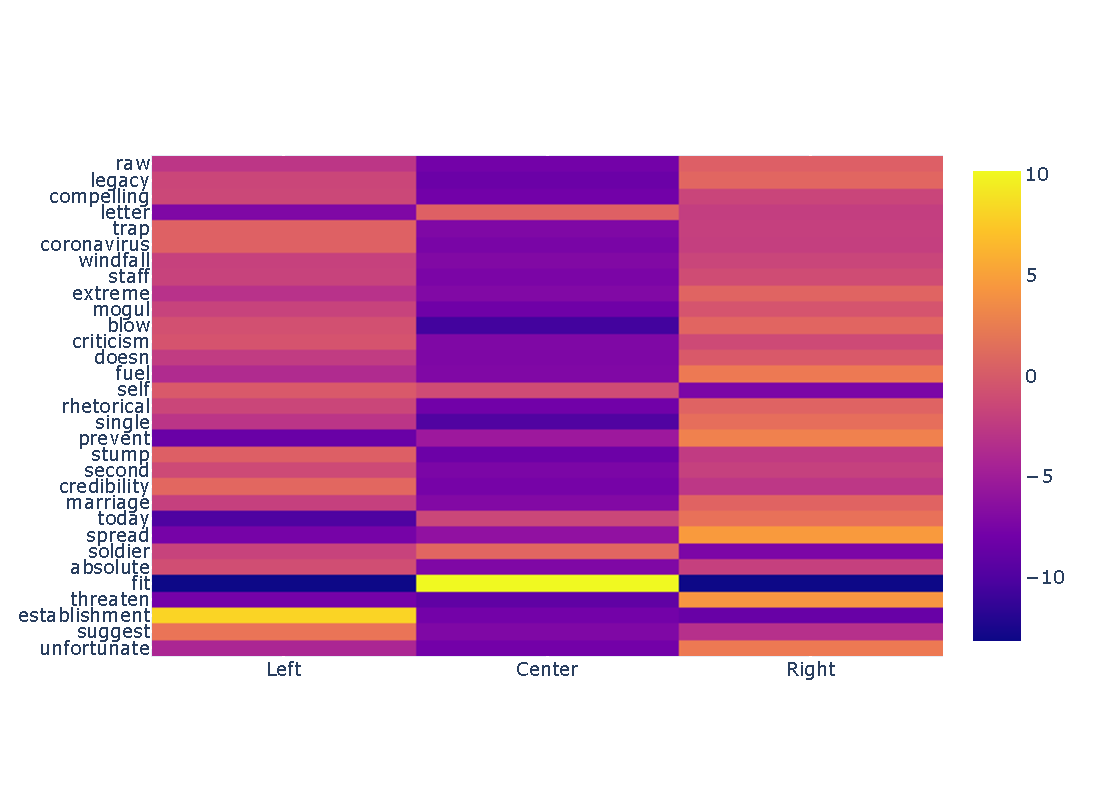
\includegraphics[width=0.75\linewidth]{figures/baly_media_weights_propaganda_tf_idf-small.pdf}
         \caption{\texttt{Prop-Total-Terms}(3a): propaganda terms}
         \label{fig:terms_weights_3a}
     \end{subfigure}
    %  \hfill
    \begin{subfigure}[b]{\linewidth}
         \centering 
         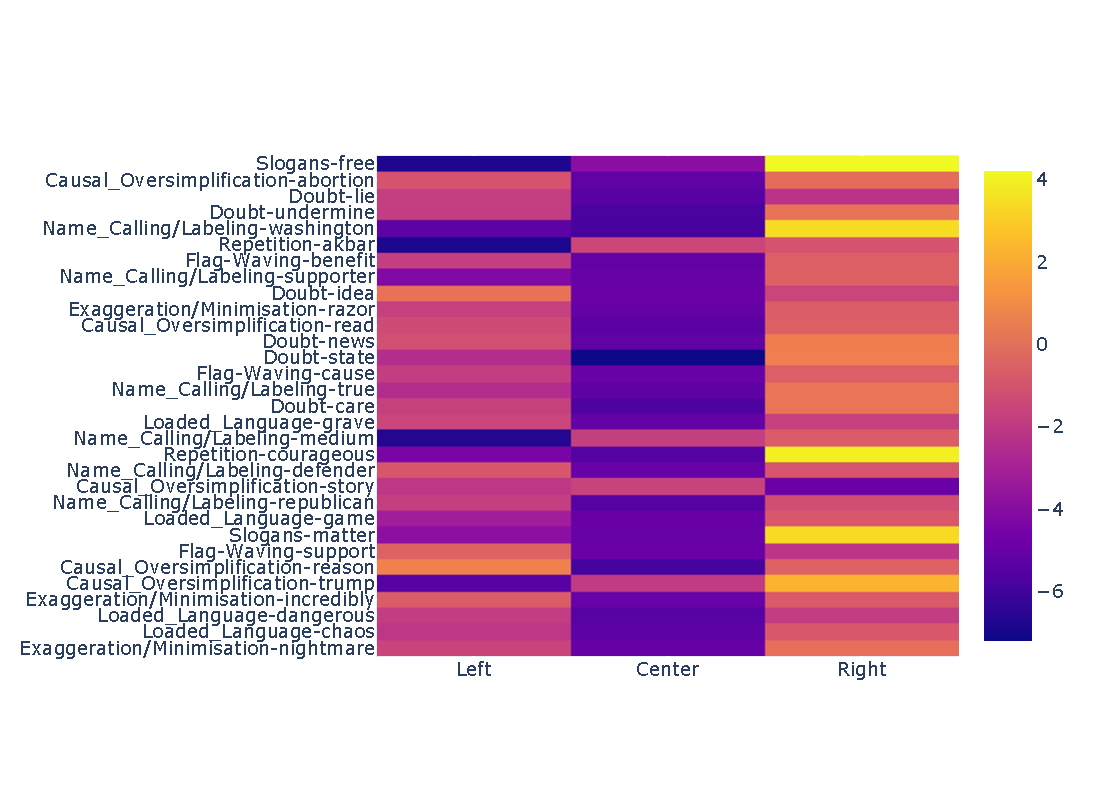
\includegraphics[width=0.75\linewidth]{figures/baly_media_weights_propaganda_techniques_tf_idf-small.pdf}
         \caption{\texttt{Prop-Techniques-Terms} (3b): propaganda terms together with their propaganda technique.}
         \label{fig:terms_weights_3b}
     \end{subfigure}
    \caption{The 30 most important terms learned by the classifier.}
    \label{fig:terms_weights}
\end{figure}

Further investigation is needed to better capture what each of these words means in the context they are used, to determine how to improve on this term analysis.% could be improved and be able to distinguish political sides more effectively.

With the current analysis, we can say that \textbf{the answer to RQ3 is a partial Yes: using as feature the terms of propaganda achieves a very similar score to the baseline (rows indicated with (3a) and (3b)), and when added to the baseline features, it helps to achieve a small (but not significant, \textit{p-value=0.657}) improvement}. % NOT SIGNIFICANT IMPROVEMENT: p-value=0.657

% TODO continue on this line!!!!



\subsubsection{Conclusion}

CIMPLE VERSION

This experiment analysed the relationship between propaganda and political leaning detection as the political leaning is an indicative factor for detecting misinformation in political context~\citep{spezzano2021s}. Using available works for propaganda detection and political leaning, we explored the effects of the propaganda features on the task of political leaning prediction. We showed that (a) propaganda is equally found in Left, Centre, and Right leaning articles, (b) detecting political leanings with propaganda features is challenging, and (c) detection performance improves when we use the amount of each propaganda technique together with the baseline features (0)+(2). The appearance of propaganda, and the techniques used, showed not to be sufficient by themselves in determining political leanings.




TTO VERSION

\paragraph{Discussion}
\begin{comment}
% Issues:

% DRAFT 1
% - data AllSides
%     - the leaning still at the author level, single articles may be from a different leaning. baly paper solution to learn the author instead of the media outlet is a step forward, but still does not represent the leaning of single articles (weak supervision). what could be done to improve it? observe alignment of viewpoint of article towards sensitive topics (pro/against): aspect-based --> my direction
% - data propaganda:
%     - propaganda corpus is only made from extreme right-leaning articles. Solution? Collect also left-leaning propaganda articles (out of scope)
%     - the propaganda annotation tool (now finally available) results in probably being biased to recognise right-leaning propaganda.
% - complexity of the task (recognising political leaning):
%     - same words used with different meaning (cit. seargeant). The context may help
%     - same techniques may be used with the same terms by opposing leanings
%     - terms/propaganda


% DRAFT 2
% Political leaning:
% - AllSides annotates at the author level (more granular than only the News Outlet level but is still distant supervision)
% - How good is the AllSides annotation? Compared to other political leanings of sources? (Media Bias/Fact Check or AdFontesMedia or Wikipedia)
% - The practical definition of political leaning: stance towards a set of topics/issues. An article from an Leftist author may contain right-leaning arguments
% POSSIBLE SOLUTION: 
% Propaganda:
% - Only extreme-right sources in the dataset of propaganda (data problem reflecting on the tool of propaganda detection)
% Intrinsic complexity of the task
% - Same words with different meaning
% - Same propaganda techniques used with same words
% - Reported speech is (should) be the same (does not depend on the news, but on the politician involved), exception of selection bias on what to be reported
\end{comment}

%%%%%% The below is to explain why not use the source. 
%Automated detection of political-leaning is still in its infancy. Although the political-leaning of articles could sometimes be gauged by their sources, there are many examples where articles' political leaning differ from that of their sources, or the sources' leanings are not well known, or the sources themselves are unknown. Hence there is a need for such detection to be based on the text of the article, rather than on where the article came from. 

In this section, we highlight various issues and directions for future work.
%present the issues that we discovered with this research. The first group relates to the political leaning, while the second one to propaganda.

\begin{comment}
% political leaning issues
%In the problems related to political leaning, we have issues that come from the data used.

%AllSides annotates at the author level. This is more granular than only the News Outlet level provided by other openly-available evaluations (such as Media Bias/Fact Check and AdFontesMedia), but it is still distant supervision.

% It also comes natural to ask how good is the AllSides annotation? Compared to other political leanings of sources, such as Media Bias/Fact Check or AdFontesMedia or Wikipedia, we can do a comparison of the leanings assigned to the sources. TODO this comparison.

This main limitation, of still annotating the leaning of the writer instead of evaluating singularly the leaning of the single articles, is probably something that needs to be analysed a bit closer.
\emph{At this point, we need to reconsider the definition of political leaning as the stance towards a set of topics/issues}. This is supported by the types of questions that are contained in surveys aimed at computing one's personal political leaning\footnote{\url{https://www.allsides.com/rate-your-bias}}. An article from a leftist author may contain right-leaning arguments.
In this work, with the third research question, we are aiming to find the terms more related to left, centre and right propaganda. Still, this analysis needs to be contextualised to be able to distinguish the same term appearing in both left and right propaganda.
% We may find discrepancies between the labels given to an article and singular pieces of text contained.
% The ground truth information could be extracted by ``AllSides Common perspectives'' \url{https://www.allsides.com/rate-your-bias} or \url{https://en.wikipedia.org/wiki/Left-wing_politics} and ``General Positions'' in  \url{https://en.wikipedia.org/wiki/Right-wing_politics}.
% Or it could also be extracted from the articles in the training set, learning the stance towards the entities like in ~\citet{chen2017opinion}.
\\

On the side of automated propaganda analysis, we need to clarify that we are using an experimental tool that therefore has many limitations.
% propaganda issues
Current work in automated propaganda analysis does not take into consideration political leaning, and seems to be focusing on Right-leaning propaganda mostly.
% Right-leaning propaganda is easier to spot because it is usually stronger and it is easier to see from the Left-perspective as opposed. There may be a bit of left-leaning in academia that facilitates this.
The results of this bias can be seen in the dataset collected by~\citet{baly2020we} (as noted in Section~\ref{ssec:related_prop}, the training of the propaganda tool is performed against right-leaning sources) and reflects on the annotations that are provided by the tool we are using. 

We acknowledge the intrinsic complexity of distinguishing left and right propaganda usage (dictated by the limitations listed above), especially if we consider that the differences we are talking about may be very subtle and challenging to pick.
For example, the same words can be used with different meaning/targets (e.g. ``enemies of the people'', ``people's will'', ...)~\cite{seargeant2020art}. This results in the same propaganda techniques used with the same words.
% % reported speech problem
% When inspecting the annotations of propaganda, we can see that a representative proportion of propaganda belongs to reported speech from public figures. In this case propaganda is not used by the reporter so we should have a method that accounts for this difference. Reported speech is (should be) the same (does not depend on the news, but on the politician involved), exception of selection bias on what to be reported.



% together issues


% The results do not bring big improvements to the State of the Art in political leaning prediction. The issues found are:

% \begin{itemize}
%     \item The effect of the features considered do not bring big improvements according to F1 and accuracy metrics. In some cases it is possible to achieve small improvements, and some of them are statistically significant. However, we want to improve the analysis and get even better results in all the cases.
%     \item Some of the models trained are probably overfitting on some small differences in the training set. Doing a comparison between the features learned and the actual distribution of the features in the dataset, we can clearly see that small differences in quantities have been amplified by the models, and this results in poor performances even on the training sets (with training accuracy observed not above 65\%)
% \end{itemize}

\end{comment}



% Limitations
\noindent\textbf{Bias in propaganda detection}: One limitation is that only articles from the Right political spectrum were used for training the propaganda detection tool provided in \cite{da2019fine}. %, which we use in our analysis. 
As we saw in our first experiment, propaganda is not limited to any particular political leaning. Therefore, propaganda annotations and model training should be less biased to a particular political leaning, and propaganda from all political directions should be used to train such models in the future, which is likely to enhance our results given our balanced dataset.  

\noindent\textbf{Baseline In/Comparability}: %with the real baseline of~\cite{baly2020we}.
As noted in Section~\ref{ssec:exp_leaning}, the shared dataset by \citet{baly2020we} differs from the one described in their paper, producing incompatibility issues between our results and theirs. %the ones they report.
Additionally, re-implementing their model could have introduced other minor differences. Therefore, we believe that comparing the results from our models with those we obtained from re-implementing the model of \citet{baly2020we} offers a fairer approach. We will repeat our tests if their model becomes available, and will continue to seek other compatible baselines once other article-specific political leaning detection models become available.  

\noindent\textbf{Meaning and Context}: As shown in experiment 3, some terminologies are common to Left, Right, and Centre articles. In political narrative, many words tend to be used frequently by different political-leaning groups, but for different meanings or to refer to different groups \cite{seargeant2020art}. For example, the word ``Elite'' is used by the Left to refer to people holding economic and political powers, and by the Right to point to those in the cultural and knowledge sector \cite{seargeant2020art}.  
Figure~\ref{fig:propaganda_example_2} shows a sentence where the \texttt{Loaded\_Language} propaganda technique was detected. In such complex examples, the structure of the discourse and framing of arguments take an essential role in discerning political leaning. 

In such cases, it might be helpful to consider propaganda techniques in relation to the surrounding context, similarly to the idea proposed in~\citet{chen2017opinion} where semantic entity analysis was used to determine opinion targets. 
All this suggests the need for a more advanced analysis on the use of certain propagandistic words by different leaning groups, to associate politically-ambiguous words with their implicit meaning, and with surrounding semantic contexts and topics.

%Annotations are costly and require experts. Automated fine-grained propaganda analysis is still at the beginning, and many issues usually come up when tools such as this are used in downstream tasks (e.g. political classification). This may be only a problem of training or it could also be a problem of different techniques that are not significant in the Right propaganda but are more prominent on the Left propaganda. More analysis on Left leaning propaganda should be done.


\begin{figure}[!tb]
    \centering
    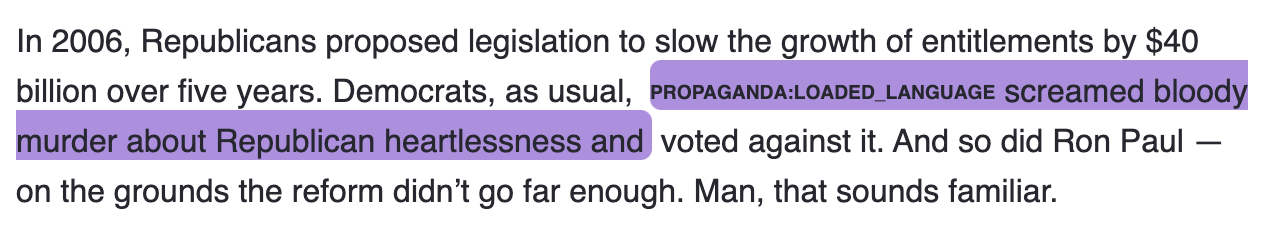
\includegraphics[width=\linewidth]{figures/propaganda_example_2.png}
    \vspace{-20px}
    \caption{An example where a propaganda technique is connected with many surrounding entities: the target of this technique are the Democrats even though the Republicans are surrounded by loaded terms.}
    \vspace{-8px}
    \label{fig:propaganda_example_2}
\end{figure}

% %%%%below is to fix a bug. if removed then figure above will not show!! 
% \begin{figure}
%     \centering
%     \includegraphics{}
%     \label{fig:my_label}
% \end{figure}

\noindent\textbf{Machine Learning Models}: In this paper, we pinned our analysis on neural network models. The additional features we calculated (e.g. TF-IDF, propaganda techniques) were added to NN models. This choice is influenced by the leading performance of such models in similar works. However, for completeness, we plan  to further test our propaganda-based features using other simpler machine learning models. %\textcolor{red}{Martino, check this plz} 

%\noindent\textbf{Context}: %features considered do not have awareness of the context.
%Articles from different political sides about the same event will naturally overlap in terminology given the shared underlining story and context. 


%Figure~\ref{fig:propaganda_example_2} shows a sentence annotation from NationalReview in which the \texttt{Loaded\_Language} propaganda technique used: ``screamed bloody murder about Republican heartlessness''. As readers, we can immediately recognise that this paragraph is pro-republican, also because there is some kind of mocking of the Democrats with the phrase ``as usual'' and the closing ``Man, that sounds familiar''.
%For recognising this automatically, similarly to what~\citet{chen2017opinion} does considering only positive vs negative sentiment, we need to mine for each entity how it has been depicted by L/C/R.
% The feature vector for every entity shows how much propaganda techniques are used together with the entity.
% For example we could learn that Right-leaning sources have the entity ``Democratic Party'' occur in sentences where loaded language is used.
%Figure~\ref{fig:propaganda_example_2} is at the same time problematic because both Democratic and Republican co-occur with loaded language (and negative sentiment).
%An improvement could be done by considering that ``Democrats'' and ``Republican'' have a different role in the sentence (subject vs object of the propaganda technique).


% This entity-specific propaganda analysis would also enable %provide interpretability of the outputs. For example, this article is from the left because it uses propaganda technique X with entity Y, which is a usual thing for articles leaning left.

% This can also be verified by comparing what has been learned with the usual position of Left and Right leaning against topics \url{https://en.wikipedia.org/wiki/Left-wing_politics}.

%%%%%%A possible problem of this approach that is not defended in the paper, is the choice of articles that have been annotated by experts. They have been selected from sources "propagandistic by Media Bias/Fact Check", in other words from the page \url{https://mediabiasfactcheck.com/fake-news/}. The propagandistic sources listed in this page, as Figure~\ref{fig:mbfc_leaning} shows, are mostly on the extreme-right side of the spectrum. Furthermore, the selection done by the authors (table 3 of that paper) results in all the sources of the articles to lean on the right.
%So the resulting model is \textbf{being trained on very propagandistic sources from the right only}. The model will not be able to see left-propaganda because it never saw it in the training phase.

\paragraph{Conclusions}
\label{sec:conclusions}
This work analysed the relationship between propaganda and political leaning detection. Using available works for propaganda detection and political leaning, we explored the effects of the propaganda features on the task of political leaning prediction. We showed that (a) propaganda is equally found in Left, Centre, and Right leaning articles, (b) detecting political-leanings with propaganda features is challenging, and (c) detection performance improves when we use the amount of each propaganda technique together with the baseline features (0)+(2).

%produced negative to mixed results. However, it also showed a small positive impact on automated political-leaning classification of articles. 

% future
The appearance of propaganda, and the techniques used, showed not to be sufficient by themselves in determining political leanings. In the next phase of this work, we plan to focus on studying the effect of propaganda features in a more contextualised approach, for example by taking into account their topics, semantic entities, and authoring country. %observing the co-occurrence of propaganda with topics and entities, and from different geographic locations. This could help in recognising the main differences is use of propaganda in relation to article topics, authoring countries, and .
% This direction is supported by observing that many times the terms of propaganda from one side overlap with the terms from the other sides, so we want to capture in this way more context around the usage of the propaganda technique.






\subsection{Other datasets for political leaning prediction}
6: classifier (propaganda → leaning) on other datasets

TODO: split this in 
1. data subsection (needed) and in
2. results of political leaning prediction subsection (previous subsection)

\subsection{\statusorange Propaganda datasets are unbalanced}
\label{ssec:ps_prop_leaning_unbalanced}

exp 8: propaganda datasets are unbalanced

RQ3: \emph{Is Propaganda Detection balanced? Or is there some imbalance in the datasets used in the literature?}

\begin{figure}[!htb]
   \centering
   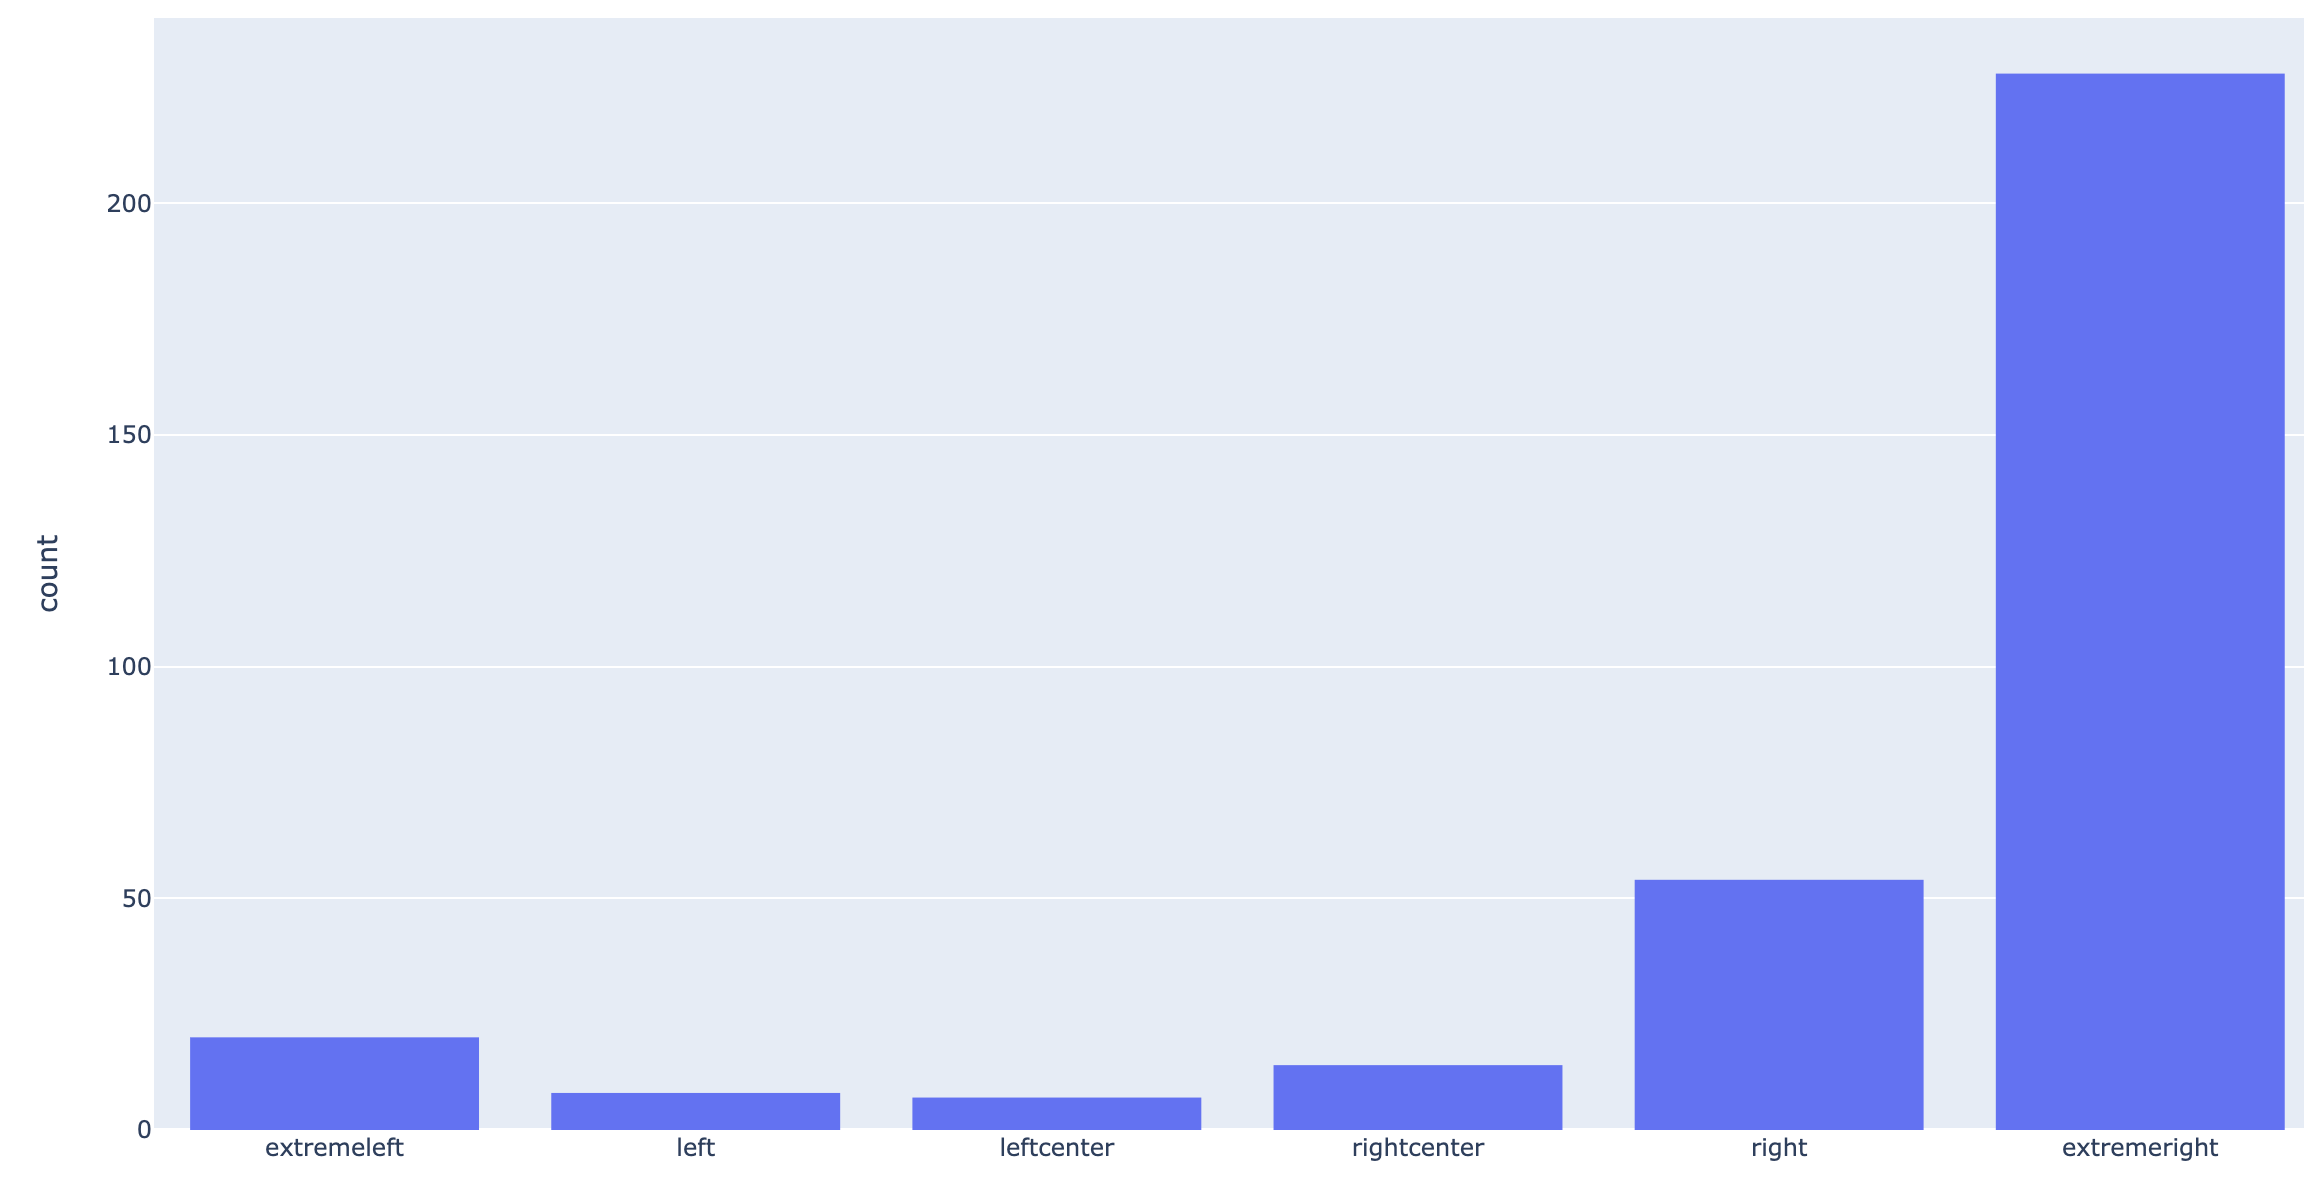
\includegraphics[width=\linewidth]{figures/leaning_questionable.png}
   \caption{The leaning of the propagandist sources from MBFC (TODO compare with effective training dataset, which is 100\% right)}
   \label{fig:mbfc_leaning}
\end{figure}

- Possible problems?
A possible problem of this approach that is not defended in the paper, is the choice of articles that have been annotated by experts. They have been selected from sources "propagandistic by Media Bias/Fact Check", in other words from the page \url{https://mediabiasfactcheck.com/fake-news/}. The propagandistic sources listed in this page, as Figure~\ref{fig:mbfc_leaning} shows, are mostly on the extreme-right side of the spectrum. Furthermore, the selection done by the authors (table 3 of that paper) results in all the sources of the articles to lean on the right.
So the resulting model is \textbf{being trained on very propagandistic sources from the right only}. The model will not be able to see left-propaganda because it never saw it in the training phase.



\subsubsection{Populism and Propaganda by leaning}

This is the continuation of Section~\ref{ssec:lp_techniques_populism_vs_propaganda} from the previous chapter. Now that we introduced the leaning and the problem of unbalance, we are going to break down the analysis with respect to the political leaning of the speeches.
% Dataset found: populism in political speeches %https://dataverse.harvard.edu/dataset.xhtml?persistentId=doi:10.7910/DVN/LFTQEZ&version=2.0 
% Each annotator (4 for each speech) gave a score between 0 (non-populistic) to 2 (very populistic)
% 4961 rows 
% 1240 deduped (352 left, 256 center, 469 right, 652 NA)
% Languages: 265 en (304 es, 148 pt, …),
% Leaning of the english ones: (36 left, 37 center, 84 right, 106 NA)

These 265 speeches all have a leaning classification (we will see more about leanings in the next chapter): 36 left, 37 center, 84 right, 106 NA. We use this information in order to check whether the results that we get are general across the political spectrum.

RESULTS

L/R evaluation:
Assumption: propaganda correlates to populism similarly in L/C/R
Result total: 0.225 Left, 0.005 Center, 0.374 Right → Why? Is it a matter of quantity of populism/propaganda?
Populism average:  [0.1259, 0.0729, 0.2712]
Propaganda average: [0.0165, 0.0271, 0.0432]
Ratio: [0.1317, 0.3717, 0.1593] → populism over propaganda ratio is a bit bigger on right (21\% more), but the correlation Right is bigger than left of 66\%. So it is less likely that this is just a matter of quantity. On the Right, propaganda and populism are strongly linked

Findings

Propaganda and populism are correlated, but not too strongly. In the Right more. This is one point supporting the hypothesis that propaganda detection works better in the Right than in the Left. → unbalanced detection caused by unbalanced data


\section{Discussions}
\label{sec:ps_discussions}

what was achieved, findings by RQ:

\begin{itemize}
    \item How does persuasion vary across the political spectrum? Less in the centre. More in the extremes. This was expected. Right seems to be more propagandistic, especially with some techniques (slogans, ...)
    \item Can we predict the political leaning of a news article by observing the propaganda it uses? Very difficult task. We see minimal effects
    \item Is Propaganda Detection balanced? Or is there some imbalance in the datasets used in the literature? Quite unbalanced datasets. Not clear what the effect of this imbalance is.
\end{itemize}

limitations

\section{Next}
\label{sec:ps_next}

Propaganda features are not enough to recognise leaning, and propaganda seems to be spread around in almost all leanings. We need to find whether, by including another dimension, we can differentiate better. 
Does it depend on the topics of the articles?

Need to break down by topic and see whether for some of them, propaganda of one leaning is very different from the one of the others.